% Soubory musí být v kódování, které je nastaveno v příkazu \usepackage[...]{inputenc}

\documentclass[%
%  draft,    				  % Testovací překlad
  12pt,       				% Velikost základního písma je 12 bodů
  a4paper,    				% Formát papíru je A4
%  oneside,      			% Jednostranný tisk (výchozí)
%% Z následujicich voleb lze použít maximálně jednu:
%	dvipdfm  						% výstup bude zpracován programem 'dvipdfm' do PDF
%	dvips	  						% výstup bude zpracován programem 'dvips' do PS
%	pdftex							% překlad bude proveden programem 'pdftex' do PDF (výchozí)
	unicode,						% Záložky a informace budou v kódování unicode
%% Z následujících voleb lze použít jen jednu:
%english,            % originální jazyk je angličtina
czech              % originální jazyk je čeština (výchozí)
%slovak,             % originální jazyk je slovenčina
]{report}				    	% Dokument třídy 'zpráva'

\usepackage[utf8]		%	Kódování zdrojových souborů je v UTF-8
	{inputenc}					% Balíček pro nastavení kódování zdrojových souborů

\usepackage{graphicx} % Balíček 'graphicx' pro vkládání obrázků
											% Nutné pro vložení log školy a fakulty

\usepackage[
	nohyperlinks				% Nebudou tvořeny hypertextové odkazy do seznamu zkratek
]{acronym}						% Balíček 'acronym' pro sazby zkratek a symbolů
											% Nutné pro použití prostředí 'seznamzkratek' balíčku 'thesis'

\usepackage[
	breaklinks=true,		% Hypertextové odkazy mohou obsahovat zalomení řádku
	hypertexnames=false % Názvy hypertextových odkazů budou tvořeny
											% nezávisle na názvech TeXu
]{hyperref}						% Balíček 'hyperref' pro sazbu hypertextových odkazů
											% Nutné pro použití příkazu 'nastavenipdf' balíčku 'thesis'

\usepackage{pdfpages} % Balíček umožňující vkládat stránky z PDF souborů
                      % Nutné při vkládání titulních listů a zadání přímo
                      % ve formátu PDF z informačního systému

\usepackage{enumitem} % Balíček pro nastavení mezerování v odrážkách
  \setlist{topsep=0pt,partopsep=0pt,noitemsep}

\usepackage{cmap} 		% Balíček cmap zajišťuje, že PDF vytvořené `pdflatexem' je
											% plně "prohledávatelné" a "kopírovatelné"

\usepackage{upgreek}	% Balíček pro sazbu stojatých řeckých písmem
											% např. stojaté pí: \uppi
											% např. stojaté mí: \upmu (použitelné třeba v mikrometrech)
											% pozor, grafická nekompatibilita s fonty typu Computer Modern!

\usepackage{dirtree}		% sazba adresářové struktury

\usepackage[formats]{listings}	% Balíček pro sazbu zdrojových textů
\lstset{
%	Definice jazyka použitého ve výpisech
%    language=[LaTeX]{TeX},	% LaTeX
%	language={Matlab},		% Matlab
	language={C},           % jazyk C
    basicstyle=\ttfamily,	% definice základního stylu písma
    tabsize=2,			% definice velikosti tabulátoru
    inputencoding=utf8,         % pro soubory uložené v kódování UTF-8
    %inputencoding=cp1250,      % pro soubory uložené ve standardním kódování Windows CP1250
		columns=fixed,  %flexible,
		fontadjust=true %licovani sloupcu
    extendedchars=true,
    literate=%  definice symbolů s diakritikou
    {á}{{\'a}}1
    {č}{{\v{c}}}1
    {ď}{{\v{d}}}1
    {é}{{\'e}}1
    {ě}{{\v{e}}}1
    {í}{{\'i}}1
    {ň}{{\v{n}}}1
    {ó}{{\'o}}1
    {ř}{{\v{r}}}1
    {š}{{\v{s}}}1
    {ť}{{\v{t}}}1
    {ú}{{\'u}}1
    {ů}{{\r{u}}}1
    {ý}{{\'y}}1
    {ž}{{\v{z}}}1
    {Á}{{\'A}}1
    {Č}{{\v{C}}}1
    {Ď}{{\v{D}}}1
    {É}{{\'E}}1
    {Ě}{{\v{E}}}1
    {Í}{{\'I}}1
    {Ň}{{\v{N}}}1
    {Ó}{{\'O}}1
    {Ř}{{\v{R}}}1
    {Š}{{\v{S}}}1
    {Ť}{{\v{T}}}1
    {Ú}{{\'U}}1
    {Ů}{{\r{U}}}1
    {Ý}{{\'Y}}1
    {Ž}{{\v{Z}}}1
}

%% Nastavení českého jazyka při sazbě v češtině.
% Pro sazbu češtiny je možné použít mezinárodní balíček 'babel', jenž
% použití doporučujeme pro nové instalace (MikTeX2.8,TeXLive2009), nebo
% národní balíček 'czech', který doporučujeme ve starších instalacích.
% Balíček 'babel' bude správně fungovat pouze ve spojení s programy
% 'latex', 'pdflatex', zatímco balíček 'czech' bude fungovat ve spojení
% s programy 'cslatex', 'pdfcslatex'.
% Varianta A:
\usepackage    				
  {babel}             % Balíček pro sazbu různojazyčných dokumentů; kompilovat (pdf)latexem!
  										% převezme si z parametrů třídy správný jazyk
\usepackage{lmodern}	% vektorové fonty Latin Modern, nástupce půvoních Knuthových Computern Modern fontů
\usepackage{textcomp} % Dodatečné symboly
\usepackage[T1]{fontenc}  % Kódování fontu - mj. kvůli správným vzorům pro dělení slov
% Varianta B:
%\usepackage{czech}   % Alternativní balíček pro sazbu v českém jazyce, kompilovat (pdf)cslatexem!

\usepackage[%
%% Z následujících voleb lze použít pouze jednu
% left,               % Rovnice a popisky plovoucich objektů budou %zarovnány vlevo
  center,             % Rovnice a popisky plovoucich objektů budou zarovnány na střed (vychozi)
%% Z následujících voleb lze použít pouze jednu
%semestral						%	sazba zprávy semestrálního projektu
bachelor						%	sazba bakalářské práce
%diploma						 % sazba diplomové práce
%treatise            % sazba pojednání o dizertační práci
%phd                 % sazba dizertační práce
]{thesis}             % Balíček pro sazbu studentských prací
                      % Musí být vložen až jako poslední, aby
                      % ostatní balíčky nepřepisovaly jeho příkazy

%\usepackage{multirow}
\usepackage{circuitikz} % circuit balicek
\makeatletter
\ctikzset{
    pir/height/.initial=1.4cm,
    pir/pitch/.initial=0.6cm,
    pir/width/.initial=0.5cm,
    pir/radius/.initial=0.5cm
}
\pgfdeclareshape{pir}{
\anchor{center}{\pgfpointorigin}
\savedanchor\topleft{%
    \pgf@y=\pgfkeysvalueof{/tikz/circuitikz/pir/pitch}
    \pgf@x=\pgfkeysvalueof{/tikz/circuitikz/pir/width}
    \pgf@x=-1.5\pgf@x
}
\anchor{power}{\topleft}
\anchor{out}{\topleft\pgf@y=0pt}
\anchor{ground}{\topleft\pgf@y=-\pgf@y}
\savedanchor\top{%
    \pgf@y=\pgfkeysvalueof{/tikz/circuitikz/pir/height}
    \pgf@y=.5\pgf@y
    \pgf@x=\pgfkeysvalueof{/tikz/circuitikz/pir/width}
    \pgf@x=-.5\pgf@x
}
\anchor{north}{\top}
\anchor{south}{\top\pgf@y=-\pgf@y}
\anchor{east}{\pgf@y=0pt\pgf@x=\pgfkeysvalueof{/tikz/circuitikz/pir/radius}}

\savedanchor\topleftbox{%
    \pgf@y=\pgfkeysvalueof{/tikz/circuitikz/pir/height}
    \pgf@y=0.5\pgf@y
    \pgf@x=\pgfkeysvalueof{/tikz/circuitikz/pir/width}
    \pgf@x=-\pgf@x
}

\foregroundpath{
    \pgfsetcolor{\pgfkeysvalueof{/tikz/circuitikz/color}}
    \pgfsetlinewidth{2\pgflinewidth} 

    \topleftbox
    \pgf@circ@res@up=\pgfkeysvalueof{/tikz/circuitikz/pir/height}
    \pgf@circ@res@up=0.5\pgf@circ@res@up
    \pgf@circ@res@down=-\pgf@circ@res@up
    \pgf@circ@res@left=\pgfkeysvalueof{/tikz/circuitikz/pir/width}
    \pgf@circ@res@left=-\pgf@circ@res@left
    \pgf@circ@res@right=0cm
    \pgfpathrectanglecorners{
        \pgfpoint{\pgf@circ@res@left}{\pgf@circ@res@down}
    }{
        \pgfpoint{\pgf@circ@res@right}{\pgf@circ@res@up}
    }
    \pgf@circ@res@right=\pgf@circ@res@left
    \pgfpathmoveto{\pgfpoint{0pt}{\pgfkeysvalueof{/tikz/circuitikz/pir/radius}}}
    \pgfpatharc{90}{-90}{\pgfkeysvalueof{/tikz/circuitikz/pir/radius}}
    \pgfusepath{draw} 
    \topleft
    \pgf@circ@res@up=\pgf@y
    \pgf@circ@res@left=\pgf@x
    \pgfpathmoveto{\pgfpoint{\pgf@circ@res@left}{ \pgf@circ@res@up}}
    \pgfpathlineto{\pgfpoint{\pgf@circ@res@right}{ \pgf@circ@res@up}}
    \pgfpathmoveto{\pgfpoint{\pgf@circ@res@left}{0pt}}
    \pgfpathlineto{\pgfpoint{\pgf@circ@res@right}{0pt}}
    \pgfpathmoveto{\pgfpoint{\pgf@circ@res@left}{-\pgf@circ@res@up}}
    \pgfpathlineto{\pgfpoint{\pgf@circ@res@right}{-\pgf@circ@res@up}}
    \pgfsetlinewidth{.5\pgflinewidth} 
    \pgfusepath{draw} 
}}
\makeatother

\usepackage{tikz}
\usepackage{smartdiagram}
\usepackage{minted}

%%%%%%%%%%%%%%%%%%%%%%%%%%%%%%%%%%%%%%%%%%%%%%%%%%%%%%%%%%%%%%%%%
%%%%%%      Definice informací o dokumentu             %%%%%%%%%%
%%%%%%%%%%%%%%%%%%%%%%%%%%%%%%%%%%%%%%%%%%%%%%%%%%%%%%%%%%%%%%%%%

%% Název práce:
%  První parametr je název v originálním jazyce,
%  druhý je překlad v angličtině nebo češtině (pokud je originální jazyk angličtina)
\nazev{Kamerový zapezpečovací systém s minipočítačem Raspberry Pi}{Camera Security System with Raspberry Pi Minicomputer}

%% Jméno a příjmení autora ve tvaru
%  [tituly před jménem]{Křestní}{Příjmení}[tituly za jménem]
\autor{Marek}{Vitula}

%% Jméno a příjmení vedoucího/školitele včetně titulů
%  [tituly před jménem]{Křestní}{Příjmení}[tituly za jménem]
% Pokud osoba nemá titul za jménem, smažte celý řetězec '[...]'
\vedouci[doc.\ Ing.]{Jaromír}{Kolouch}[CSc.]

%% Jméno a příjmení oponenta včetně titulů
%  [tituly před jménem]{Křestní}{Příjmení}[tituly za jménem]
% Pokud nemá titul za jménem, smažte celý řetězec '[...]'
% Uplatní se pouze v prezentaci k obhajobě;
% v případě, že nechcete, aby se na titulním snímku prezentace zobrazoval oponent, pouze jej zakomentujte;
% u obhajoby semestrální práce se oponent nezobrazuje
\oponent[doc.\ Mgr.]{Křestní}{Příjmení}[Ph.D.]

%% Označení oboru studia
% První parametr je obor v originálním jazyce,
% druhý parametr je překlad v angličtině nebo češtině
\oborstudia{Elektronika a sdělovací technika}{Electronics and Communications}

%% Označení fakulty
% První parametr je název fakulty v originálním jazyce,
% druhý parametr je překlad v angličtině nebo v češtině
%\fakulta{Fakulta architektury}{Faculty of Architecture}
\fakulta{Fakulta elektrotechniky a komunikačních technologií}{Faculty of Electrical Engineering and Communication}
%\fakulta{Fakulta chemická}{Faculty of Chemistry}
%\fakulta{Fakulta informačních technologií}{Faculty of Information Technology}
%\fakulta{Fakulta podnikatelská}{Faculty of Business and Management}
%\fakulta{Fakulta stavební}{Faculty of Civil Engineering}
%\fakulta{Fakulta strojního inženýrství}{Faculty of Mechanical Engineering}
%\fakulta{Fakulta výtvarných umění}{Faculty of Fine Arts}

%% Označení ústavu
% První parametr je název ústavu v originálním jazyce,
% druhý parametr je překlad v angličtině nebo češtině
%\ustav{Ústav automatizace a měřicí techniky}{Department of Control and Instrumentation}
%\ustav{Ústav biomedicínského inženýrství}{Department of Biomedical Engineering}
%\ustav{Ústav elektroenergetiky}{Department of Electrical Power Engineering}
%\ustav{Ústav elektrotechnologie}{Department of Electrical and Electronic Technology}
%\ustav{Ústav fyziky}{Department of Physics}
%\ustav{Ústav jazyků}{Department of Foreign Languages}
%\ustav{Ústav matematiky}{Department of Mathematics}
%\ustav{Ústav mikroelektroniky}{Department of Microelectronics}
\ustav{Ústav radioelektroniky}{Department of Radio Electronics}
%\ustav{Ústav teoretické a experimentální elektrotechniky}{Department of Theoretical and Experimental Electrical Engineering}
%\ustav{Ústav telekomunikací}{Department of Telecommunications}
%\ustav{Ústav výkonové elektrotechniky a elektroniky}{Department of Power Electrical and Electronic Engineering}

\logofakulta[loga/FEKT_zkratka_barevne_PANTONE_CZ]{loga/UTKO_color_PANTONE_CZ}


%% Rok obhajoby
\rok{2018}
\datum{13.\,12.\,2017} % Datum se uplatní pouze v prezentaci k obhajobě

%% Místo obhajoby
% Na titulních stránkách bude automaticky vysázeno VELKÝMI písmeny
\misto{Brno}

%% Abstrakt
\abstrakt{Tato bakalářská práce se zabývá návrhem kamerového zabezpečovacího systému na platformě Raspberry Pi. V první části popisuje jednotlivé hardwarové a softwarové komponenty, které budou použity pro zařízení. V druhé části se práce zabývá návrhem aplikace pro detekci pohybu z obrazu a též pomocí pohybového čidla PIR a následného zpracování dat a odeslání na cloudové úložiště. Závěrečná část práce se věnuje hardwarové části, především návrhu napájení zařízení akumulátorem, který je dobíjen ze solárního panelu a také návrhu tranzistorového spínače pro výkonovou LED.}
{This bachelor thesis describes a design of a camera surveillance system on the Raspbery Pi platform. First part of the thesis describes the individual hardware and software components to be used for the device. Second part deals with the design of the actual application for motion detection using the output from the camera and PIR motion sensor and the following processing and sending data to a cloud storage. The final part of the thesis describes the design of the hardware, particularly solar panel and battery and also the design of the power LED switch.}

%% Klíčová slova
\klicovaslova{Raspberry Pi, kamera, počítačové vidění, solární napájení, Python, Linux }%
	{Raspberry Pi, camera, computer vision, solar powered, Python, Linux}

%% Poděkování
\podekovanitext{Rád bych poděkoval vedoucímu bakalářské práce panu doc. Ing. Jaromírovi Kolouchovi, CSc.\ a odbornému konzultantovi panu Ing. Ondřejovi Pavelkovi\ za odborné vedení, trpělivost při konzultacích a jejich podnětné návrhy k~mé práci.}  % do tohoto souboru doplňte údaje o sobě, o názvu práce...

%%%%%%%%%%%%%%%%%%%%%%%%%%%%%%%%%%%%%%%%%%%%%%%%%%%%%%%%%%%%%%%%%%%%%%%%

%%%%%%%%%%%%%%%%%%%%%%%%%%%%%%%%%%%%%%%%%%%%%%%%%%%%%%%%%%%%%%%%%%%%%%%%
%%%%%%     Nastavení polí ve Vlastnostech dokumentu PDF      %%%%%%%%%%%
%%%%%%%%%%%%%%%%%%%%%%%%%%%%%%%%%%%%%%%%%%%%%%%%%%%%%%%%%%%%%%%%%%%%%%%%
%% Při vloženém balíčku 'hyperref' lze použít příkaz '\nastavenipdf'
\nastavenipdf
%  Nastavení polí je možné provést také ručně příkazem:
%\hypersetup{
%  pdftitle={Název studentské práce},    	% Pole 'Document Title'
%  pdfauthor={Autor studenstké práce},   	% Pole 'Author'
%  pdfsubject={Typ práce}, 						  	% Pole 'Subject'
%  pdfkeywords={Klíčová slova}           	% Pole 'Keywords'
%}
%%%%%%%%%%%%%%%%%%%%%%%%%%%%%%%%%%%%%%%%%%%%%%%%%%%%%%%%%%%%%%%%%%%%%%%

%%%%%%%%%%%%%%%%%%%%%%%%%%%%%%%%%%%%%%%%%%%%%%%%%%%%%%%%%%%%%%%%%%%%%%%
%%%%%%%%%%%       Začátek dokumentu               %%%%%%%%%%%%%%%%%%%%%
%%%%%%%%%%%%%%%%%%%%%%%%%%%%%%%%%%%%%%%%%%%%%%%%%%%%%%%%%%%%%%%%%%%%%%%
\begin{document}


%% Vložení desek generovaných informačním systémem
\includepdf[pages=1,offset=15.4mm -1in]%
  {pdf/student-desky}% název souboru nesmí obsahovat mezery!
% nebo vytvoření desek z balíčku
%\vytvorobalku
\setcounter{page}{1} %resetovani citace stranek - desky se necisluji

%% Vložení titulního listu generovaného informačním systémem
\includepdf[pages=1,offset=15.4mm -1in]%
  {pdf/student-titulka}% název souboru nesmí obsahovat mezery!
% nebo vytvoření titulní stránky z balíčku
%\vytvortitulku
   
%% Vložení zadání generovaného informačním systémem
\includepdf[pages=1,offset=15.4mm -1in]%
  {pdf/student-zadani}% název souboru nesmí obsahovat mezery!
% nebo lze vytvořit prázdný list příkazem ze šablony
%\stranka{}%
%	{\sffamily\Huge\centering ZDE VLOŽIT LIST ZADÁNÍ}%
%	{\sffamily\centering Z~důvodu správného číslování stránek}

%% Vysázení stránky s abstraktem
\vytvorabstrakt

%% Vysázení prohlaseni o samostatnosti
\vytvorprohlaseni

%% Vysázení poděkování
\vytvorpodekovani

%% Vysázení poděkování projektu SIX
% ----------- zakomentujte pokud neodpovida realite
%\vytvorpodekovaniSIX

%% Vysázení obsahu
\obsah

%% Vysázení seznamu obrázků
\seznamobrazku

%% Vysázení seznamu tabulek
\seznamtabulek

%% Vysázení seznamu výpisů
\lstlistoflistings

%% Vložení souboru 'text/uvod.tex' s úvodem
\chapter*{Úvod}
\phantomsection
\addcontentsline{toc}{chapter}{Úvod}


Tento dokument popisuje semestrální práci vytvořenou na VUT, fakultě elektrotechniky, v Brně.

Po krátkém úvodu a seznámení se zadáním práce následuje kapitola číslo 1, ve které je popsán minipočítač Raspberry Pi, na kterém bude práce dále stavět. Dále je popsán operační systém Raspbian a další 
programové vybavení, které bude použito. Je zde teoreticky popsán způsob detekce pohybu a také je teoreticky objasněn problém solárního napájení.

Kapitola č. 2 popisuje návrh aplikace pro detekci pohybu.

Návrh řešení se nachází v kapitole č. 3 a popis samotné realizace projektu je v kapitole č. 4.  

Poslední kapitola krátce hodnotí celou práci a navrhuje případná zlepšení.

\section*{Úvod do problematiky}
Práce si klade za cíl vytvořit zařízení, které bude schopné sloužit jako monitorovací systém, například pro ostrahu objektu, nebo pro monitorování zvěře.

Ve srovnání s komerčně dostupnými, kamerovými zabezpečovacími systémy, bude navrhovaný systém, vytvořený na platformě Raspberry Pi a Linux, disponovat větší variabilitou.

Monitorovací systém je navržen tak, aby mohl být po nějakou dobu energeticky soběstačný. Problém lze řešit napájením pomocí solárního panelu, kterým bude dobíjen akumulátor.

Systém by tedy měl být energeticky úsporný. Bude nutné vybrat vhodnou, spolehlivou metodu detekce obrazu, která by nevyžadovala pro svoji činnost příliš mnoho elektrické energie.

Konektivita monitorovacího systému do sítě Internet bude zajištěna pomocí přídavného modulu. 

%% Vložení souboru 'text/reseni' s popisem reseni práce
\chapter[Teoretická část práce]{Teoretická část práce}

\section{Hardwarové vybavení}

\subsection*{Raspberry Pi}
Raspberry Pi je název malého, jednodeskového počítače vyvinutého britskou nadací Raspberry Pi Foundation v roce 2012 s cílem podpořit výuku informatiky a vytvořit počítač dostupný pro všechny. V roce 2017 byla dostupná již třetí generace tohoto minipočítače a také zmenšená verze Raspberry Pi Zero a Zero W.

Primárním operačním systémem je Raspbian, což je derivát Linuxu Debianu, avšak je možné použít i řadu jiných operačních systémů, například Windows IoT Core nebo RISC OS.\cite{rpidoc}

\subsubsection{Raspberry Pi Zero W}
Základem Raspberry Pi Zero W je SoC (System on a chip) Broadcom BCM2835 založený na 32 bitové architektuře ARMv6. Taktovací frekvence procesoru je 1 GHz.

Počítač je vybaven 512 MB paměti typu SDRAM a grafickým procesorem Broadcom Videocore IV. Pro úložiště dat jsou použity microSD karty.

Doporučená cena v době uvedení na trh byla 10 USD.\cite{rpidoc}

\begin{figure}[h]
  \begin{center}
    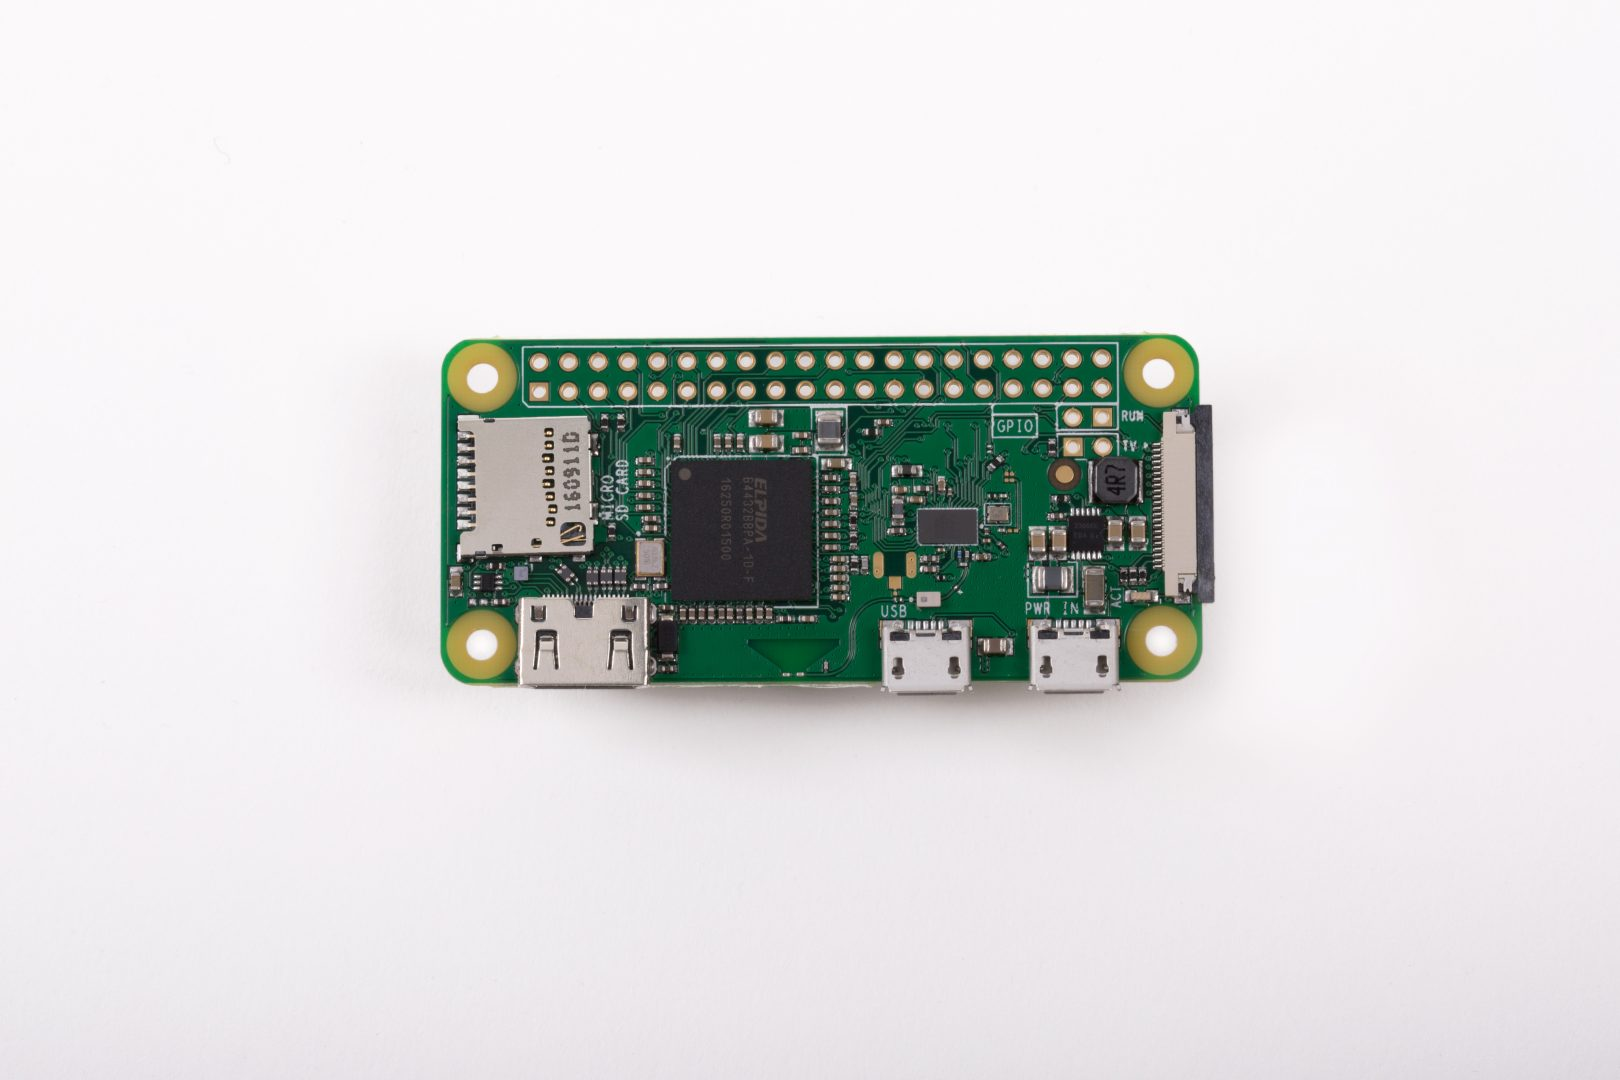
\includegraphics[scale=0.3]{obrazky/rpizero.jpg}
  \end{center}
  \caption{Raspberry Pi Zero W, převzato z thepihut.com}
\end{figure}

\subsubsection{Napájení a spotřeba}
Zařízení je napájeno z micro USB portu napájecím napětím 5V. Dle technické dokumentace se proudový odběr ve stavu nečinnosti pohybuje kolem 100 mA. Maximální odběr zařízení včetně zapojené klávesnice, myši a obrazovky může být až 350 mA.

Nicméně lze různými postupy snížit proudový odběr až na 80 mA ve stavu nečinnosti. Například vypnutím HDMI portu se odběr sníží o 25 mA, vypnutí LED diod ušetří až 5 mA.
Spotřeba elektrické energie také velmi záleží na počtu připojených perifierií. Samostatná Python kamera má spotřebu přibližně 250 mA.

Velký vliv na spotřebu má také vytížení procesoru.
Bude tedy vhodné optimalizovat algoritmus detekce obrazu tak, aby využíval co nejméně procesorového času a ve výsledku spotřeboval co nejméně elektrické energie.

\subsubsection{GPIO}
GPIO je zkratka pro General Purpose Input Output. Jsou to uživatelsky konfigurovatelné piny, které mohou být jak vstupní, tak výstupní. Raspberry Pi Zero, Raspberry Pi 3 a Raspberry Pi 2 disponuje 40 takovými piny. Pro srovnání - první verze Raspberry Pi A a B disponovala pouze 26 těmito piny.

Raspberry Pi používá 3,3voltovou logiku, je tedy nutné použít pro zapojení periferií využívajících 5 V převodník úrovní.

GPIO je možné nastavit například jako UART, SPI, I2C nebo PCM.

Pro ovládání GPIO lze použít Python modul GPIO, který ale v době psaní práce (verze 0.63) umožnil pouze softwarové GPIO. Nebylo tedy například umožněno hardwarové generování PWM signálu.

Pro hardwarové generování signálu lze využít modul RPIO, který umožňuje generování PWM pomocí DMA s přesností 1,2 mikrosekundy.

\begin{figure}[!h]
  \begin{center}
    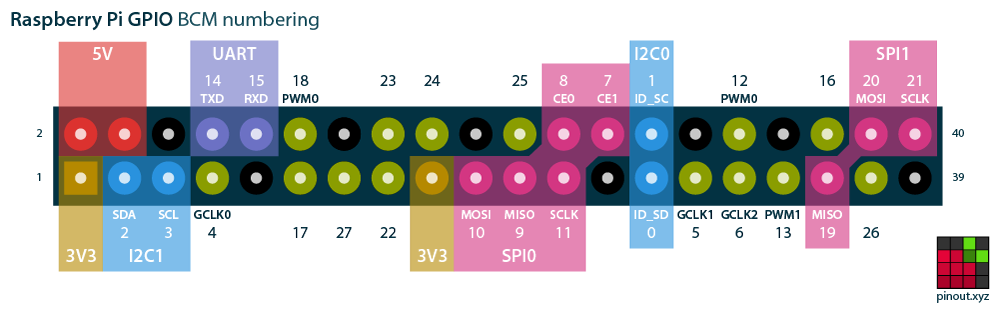
\includegraphics[scale=0.41]{obrazky/raspberry-pi-pinout.png}
  \end{center}
  \caption{Raspberry Pi GPIO Pinout, převzato z pinout.xyz}
\end{figure}

\subsubsection{Úložiště}
Raspberry Pi standardně používá jako úložiště (micro)SD karty. Maximální propustnost čtečky karet je 25 MB/s, je dána omezením sběrnice USB.

Spotřebitelské SD karty používají levné paměti typu TLC. Berme tedy v úvahu, že spotřebitelské SD karty mají kratší životnost než při užití pevného disku. K dostání jsou ale i karty pro průmyslové použití, které využívají pamětí typu MLC či SLC, které mají několikanásobně vyšší životnost než TLC paměti.

Životnost paměti se dá zvýšit například použitím RAM disku tmpfs v Linuxu. Také je možné přesunout root na jiný typ úložiště a SD kartu ponechat pouze na bootování.

Při preferenci co nejnižší spotřeby elektrické energie monitorovacího zařízení, bude vhodné použít jako hlavní datové úložiště pouze SD kartu.

\subsection*{Raspberry Pi NoIR Camera Board V2}
Vzhledem k požadavku na noční snímání je použita kamera bez infračerveného filtru Raspberry Pi NoIR Camera Board V2. Kvůli absenci IR filtru je možné využití okem neviditelného infračerveného přísvitu.

\begin{figure}[h]
  \begin{center}
    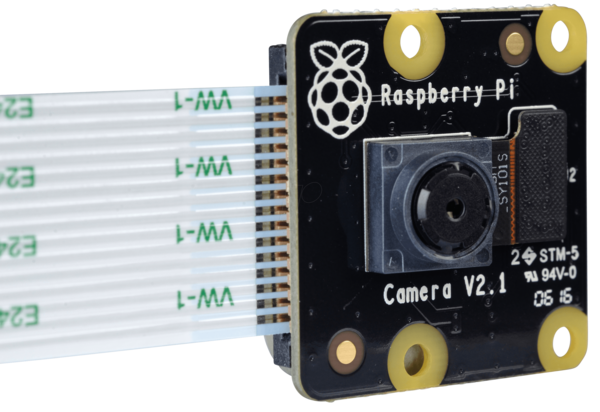
\includegraphics[scale=0.3]{obrazky/rpicamera.png}
  \end{center}
  \caption{Raspberry Pi NoIR Camera V2, převzato z reichelt.de}
\end{figure}

Kamera disponuje 8 megapixelovým obrazovým senzorem Sony IMX219 a fixním ohniskem. Videa je možné natáčet až do rozlišení 1920x1080 pixelů při 30 fps a je možné pořizovat statické snímky až do rozlišení 3820x2464 pixelů.

Zorné pole kamery v horizontálním směru je 62 úhlových stupňů.

Kamera je připojena pomocí vysokorychlostního sériového rozhraní CSI, které má ve verzi 3 teoretickou maximální datovou propustnost 5,8 Gbps.

\begin{figure}[!h]
  \begin{center}
    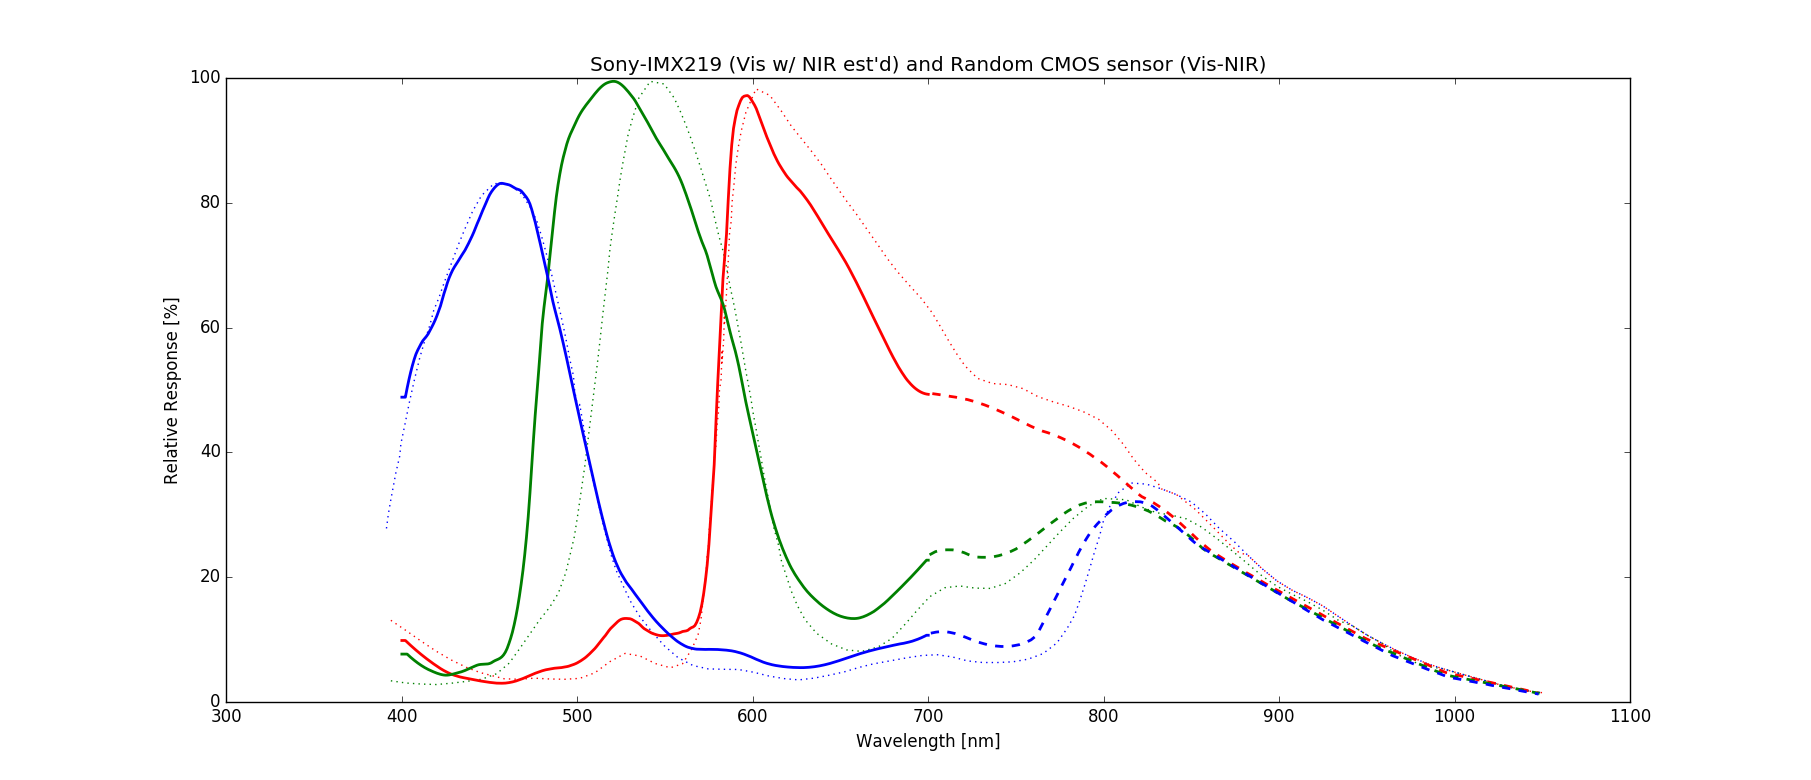
\includegraphics[scale=0.32]{obrazky/SonyIMX219approx.png}
  \end{center}
  \caption{Aproximovaná spektrální citlivost CMOS snímače Sony IMX219. Autorem je Koen Hufkensem  \cite{sony}}
\end{figure} 
Data zobrazena plnou čarou zobrazují spektrální citlivost ve viditelném spektru a jsou extrahovány z datasheetu produktu.

Data zobrazena přerušovanou čarou jsou aproximována porovnáním spektrální citlivosti podobného CMOS snímače od firmy Sony.

Z grafu tedy vyplývá, že citlivost snímače klesá se prodlužující se vlnovou délku světla, které dopadá na snímač CMOS. Přibližně při vlnové délce světla 1050 nm je spektrální citlivost snímače rovna téměř nulová.

Tuto informaci můžeme využít k nákupu vhodné infračervené diody pro přísvit kamery, aby bylo zajištěno dobré snímání obrazu při nevhodných světelných podmínkách.

\subsection*{GSM/GPRS modul SIM800}
SIM800 je modul od společnosti SIMCom pro bezdrátovou komunikaci pomocí technologie GSM a GPRS.

Podporuje frekvenční pásma 850/900/1800/1900 MHz, hlasovou komunikaci, SMS a GPRS data třídy 10.

Maximální teoretická přenosová rychlost pro CS4 je tedy 85,6 kbps pro downlink a 21,4 kbps pro uplink. Ke komunikaci je možné využít sériové rozhraní podporující AT příkazy, nebo je možné využít PPP stack pro internetové připojení.

Pro připojení k Raspberry Pi využijeme sériovou sběrnici UART. Modul podporuje baudovou rychlost od 1200 do 460800 Bd. 

\subsubsection{Point-to-Point Protocol}
Point-to-Point Protocol, zkráceně PPP je název komunikačního protokolu linkové vrstvy, používaný pro přímé spojení mezi dvěma síťovými uzly.

V našem případě budeme tento protokol používat pro navázání spojení mezi GPRS modulem po sériové lince. K připojení je použit program PPPD, který naváže spojení pomocí tzv. chatovacích skriptů.

\subsubsection{AT příkazy}
AT příkazy jsou instrukce pro řízení modemu. AT je zkratka pro ATention.

Každý příkaz začíná "AT". Jako příklad uveďme příkazy specifické pro komunikaci s GSM/GPRS modemem: AT+CMGS je příkaz pro odesílání SMS zprávy, AT+CGSN je příkaz pro získání IMEI čísla modemu.

\subsubsection{APN}
APN, neboli Access Point Name je jméno brány mezi sítí GSM/GPRS a sítí Internet. Název APN pro daného mobilního operátora nám musí být znám před připojením.

\subsection*{PIR modul HC-SR501}
Modul HC-SR501 používá PIR element LHI778 a integrovaný obvod BISS0001 pro obsluhu signálu z PIR elementu.

Modul umožňuje nastavení citlivosti snímání v rozsahu od 3 do 7 metrů vzdálenosti snímaného objektu od kamery a také nastavení časového zpoždění mezi detekovaným pohybem a odeslaným signálem o detekci.

Nastavení citlivosti snímání je prováděno pomocí potenciometru na modulu.

Napájecí napětí je v rozmezí 5 až 20 V. Pokud je detekován pohyb, objeví se na výstupním pinu logická jednička (3,3 V), která zůstane aktivní po nastavenou dobu.

Nastavení časového zpoždění je též prováděno potenciometrem.

Po vypršení nastaveného zpoždění, zůstane modul ještě 2,5 sekundy ve stavu logické nuly.

V tomto 2,5 sekundovém časovém úseku nemůže být detekován další pohyb snímaného objektu.

Modul může pracovat ve dvou režimech detekce pohybu, buď v jednoduchém nebo opakovaném.

V jednoduchém režimu dojde k zahájení odpočítávání časovače zpoždění ihned po detekci pohybu. K dalšímu restartování může dojít až po vypršení nastaveného času.

V opakovaném režimu je časovač restartován s každým dalším detekovaným pohybem.

\begin{table}[h]
\centering
\caption{Možnosti modulu HC-SR501}
\label{HC-SR501}
\begin{tabular}{|l|l|}
\hline
\textbf{Pin nebo nastavení} & \textit{Funkce}                                            \\ \hline
Zpoždění            & Jak dlouho má být na výstupním pinu logická 1                     \\ \hline
Citlivost           & Rozsah nastavení vzdálenosti od 3 m až 7 m                                   \\ \hline
Spouštění           & Jednoduché nebo opakované zpoždění.                               \\ \hline
GND                 & Uzemnění                                                          \\ \hline
Výstup              & Logický výstup 3,3 V, pokud je detekován pohyb                     \\ \hline
Napájení            & 5 až 20 V DC napětí                                                \\ \hline
\end{tabular}
\end{table}

\begin{figure}[!h]
  \begin{center}
   \begin{circuitikz} 
        \draw (0,0) node[pir] (pir) {}
            (pir.power) node[anchor=east] {Napájení}
            (pir.ground) node[anchor=east] {GND}
            (pir.out) node[anchor=east] {Výstup}
            (pir.north) node[anchor=south] {}
            (pir.south) node[anchor=north] {}
            (pir.east) node[anchor=west] {};
\end{circuitikz} 
  \end{center}
  \caption{Schéma PIR modulu}
\end{figure}


\subsection*{Výkonová IR LED dioda GT-P04IR4101}
\subsubsection{Parametry}
\begin{table}[h]
\centering
\caption{Parametry LED z katalogu}
\label{Parametry LEDl}
\begin{tabular}{|l|l|l|l|}
\hline
\textbf{Parametr}        & \textit{min.} & \textit{typická} & \textit{max.} \\ \hline
Ztrátový výkon &              & 1 W           &              \\ \hline
Úbytek napětí            & 1,65 V        &              & 1,75 V        \\ \hline
Proudový odběr            &              & 400 mA        & 420 mA             \\ \hline
Vyzářený výstupní výkon      &              & 400 mW        &              \\ \hline
Vlnová délka světla         &              & 850 nm        &              \\ \hline
Tepelný odpor         &              & 12 °C/W       &              \\ \hline
Úhel osvětlení              &              & 120°         &              \\ \hline
\end{tabular}
\end{table}

\clearpage


\section{Programové vybavení}

\subsection*{Raspbian}
Raspbian je linuxový operační systém založený na distribuci Debian. Je optimalizovaný pro hardware Raspberry Pi, určený pro architekturu armhf. První verze byla vytvořena v roce 2012. Raspbian bude použit ve verzi lite, tedy bez grafického rozhraní a pouze s nutnými programovými knihovnami - balíčky.

\subsection*{Python}
Python je vysokoúrovňový skriptovací jazyk navržený Guidem Van Rossem v roce 1991.
Jazyk podporuje několik programovacích paradigmat včetně objektového, procedurálního a funkcionálního. V roce 2017 existovaly dvě navzájem částečně nekompatibilní odnože Pythonu a to 2.7.x a 3.x.x. Python je snadno rozšířitelný o další programové knihovny - balíčky.

\subsubsection{Picamera}
Picamera je knihovna pro Python, která umožňuje ovládat kameru pro Raspberry Pi, včetně pořizování statických snímků a videí. Poskytuje poměrně bohaté programové API.

\subsubsection{Pillow}
Pillow je knihovna pro Python, která vznikla jako derivát staršího modulu PIL. Pillow rozšiřuje schopnosti Pythonu o pokročilé zpracování obrazu.

\subsubsection{PyDrive}
PyDrive je knihovna pro Python pro práci s cloudovým úložištěm Google Drive. Vznikla jako zjednodušení Google Drive REST API. Knihovna umožňuje jednoduchou manipulaci se soubory uloženými na Google Drive. K autentizaci uživatele je použit framework OAuth 2.

\subsubsection{Python-gsmmodem}
Python-gsmmodem je knihovna pro Python pro komunikaci s modemy pomocí AT příkazů. Podporuje odesílání a příjmání SMS zpráv a také hlasovou telefonii.

\subsubsection{Epsolar-tracer}
Epsolar-tracer je knihovna pro Python pro komunikaci se solárním regulátorem Epsolar využívající protokol Modbus a rozhraní RS-485. Knihovna je použita pro komunikaci mezi Raspberry Pi a solárním regulátorem.

\subsection*{Google Apps Script}
Google Apps Script je skriptovací jazyk založený na Java Scriptu pro webové aplikace běžící pod Google Cloudem. Google poskytuje běhové prostředí a editor s debuggerem. V projektu je tento jazyk využíván pro vytvoření grafického rozhraní pro konfiguraci aplikace a pro sběr dat.

\subsection*{JSON}
JSON je zkratka pro JavaScript Object Notation. Je to jednoduchý formát pro výměnu dat. Jeho výhoda spočívá v tom, že má jednoduchou strukturu. Je tedy lehce čitelný i lehce editovatelný a má také velmi dobrou podporu v programovacích jazycích. V projektu je tento formát využíván pro konfiguraci aplikace.

\subsection*{Závěr k výběru softwaru}
Veškeré vybrané softwarové vybavení se řadí do kategorie Open-source. Takový software je vyvíjen především komunitně a jeho zdrojový kód je volně k dispozici. Cena softwaru je tedy nulová.
Další kapitola se bude zabývat využitím vybraného softwaru.

\section{Detekce pohybu}
Detekce pohybu je proces detekce změny pozice zkoumaného objektu vůči pozadí. Zde se budeme zabývat především elektronickou detekcí pohybu.

Existuje několik metod elektronické detekce pohybu, například optická nebo akustická metoda. Mezi optické metody patří detekce infračerveného záření pomocí PIR senzoru. Příklad akustické metody je detekce ultrazvukem.

\subsection*{Pohyb}
Pod pojmem pohyb rozumíme pohyb mechanický, což je změna polohy pozorovaného objektu.
Pohyb nelze detekovat z jednoho statického obrazu, potřebujeme obrazový tok.
Budeme tedy pracovat s dynamickým obrazem, což je posloupnost statických obrazů.

\subsection*{Detekce pohybu pomocí PIR senzoru}
Zkratka PIR znamená „passive infrared“, jde tedy o pasivní infračervený detektor, který funguje na principu pyroelektrického jevu.

\subsection*{Pyroelektrický jev}
Pyroelektrický jev je schopnost materiálu generovat dočasný elektrický potenciál při změně teploty. Vyskytuje se u dielektrik s jednou polární osou symetrie.

\subsection*{PIR Element}
PIR element je základní funkční prvek PIR detektoru. Je to polovodičová součástka, citlivá na světlo, vyrobená ze sloučenin na bázi lithia a tantalu. PIR snímač je citlivý v širokém spektru záření, je proto nutné před snímač aplikovat filtr, který propouští pouze infračervené záření o vlnových délkách v rozsahu 8 až 14 $\jedn{\mu m}$. Lidské tělo emituje záření o vlnové délce 9,4 $\jedn{\mu m}$. Se změnou intenzity dopadajícího infračerveného záření na povrch pyroelektrického materiálu se změní hodnota elektrického povrchového náboje. Tato změna je měřena citlivým tranzistorem FET. \cite{pir_senzor}

\subsection*{Optika}
Úkolem optické soustavy je soustřeďovat infračervené záření z detekční zóny do PIR elementu. V praxi se používají Fresnelovy čočky nebo zrcadla.

\subsection*{Detekce pohybu z dynamického obrazu}
Existuje několik metod pro detekci pohybu ze snímané scény.
Metody jsou primárně založené na segmentaci pozadí a popředí obrazu.
Pozadím nazýváme část obrazu ve které zjišťujeme změny a popředí nese právě ty změny. Pozadí ale většinou nebývá statické, je v něm obsažen například šum snímacího zařízení, nebo změny osvětlení. 

Je několik algoritmů, které tyto problémy řeší s různými nároky na výpočetní výkon.

Zmiňme například:
\begin{itemize}
    \item
    Porovnávaní histogramu mezi snímky
    \item
    Sledování rozdílných bodů mezi snímky
    \item
    Porovnání snímků zpracovaných detektorem hran
    \item
    Metoda optického toku
    \item
    GMM - Gaussian Mixture Models
    \item
    Sigma-Delta filtrace
\end{itemize}

\subsection*{Porovnávání histogramu mezi snímky}
Jedná se o jednu z nejjednodušších metod detekce pohybu. Porovnávají se histogramy dvou snímků - vyhodnocují se tedy jasové charakteristiky snímků. Tato metoda je výpočetně málo náročná a je vhodná pouze do podmínek se stálým osvětlením. Je nutné dobře zvolit referenční snímek podle kterého se bude porovnávat pohyb a průběžně ho aktualizovat podle změn v prostředí. Výpočetně nejméně náročné je průměrování histogramů několika snímků, ve kterých není označen pohyb. Také je dobré snímek zbavit šumu přes šumové filtry. \cite{fbmi_video}

\subsubsection{Výhody} 
Výpočetně málo náročná metoda.
\subsubsection{Nevýhody}
Metoda je náchylná na šum a také na změny prostředí.

\subsection*{Sledování rozdílných bodů mezi snímky}
Tato metoda spočívá v porovnáváni snímků na úrovni pixelů. Je vhodné snímky nejprve převést do 8-bitového barevného prostoru a potom odečítat hodnoty.  Obrázky od sebe v této podobě odečteme a získáme nový snímek, který nyní bude prezentovat rozdíl složek. Čím méně se od sebe korespondující pixely liší, tím se jejich hodnota v rozdílu bude více blížit hodnotě 0 (černá barva). Poté je nutné aplikovat metodu prahování abychom rozeznali informaci od šumu. \cite{fbmi_video}
\subsubsection{Výhody}
Schopnost určit místo ve scéně na kterém došlo k pohybu.
\subsubsection{Nevýhody}
Relativně výpočetně náročná operace porovnávání snímků na úrovni pixelů.

\subsection*{Metoda optického toku}

Metoda optického toku dokáže sledovat pohyb pixelu mezi snímky ve video sekvenci a zjistit tak rychlost pohybu. Tímto způsobem se dá předpovídat trajektorie sledovaného objektu. Metoda je výpočetně velmi náročná pro sledování všech pixelů ve scéně. S určitou optimalizací je však použitelná i jako detektor pohybu. 

\section{Mobilní sítě}
\subsection*{GSM}
GSM (Groupe Spécial Mobile) popisuje protokoly pro mobilní telekomunikaci druhé generace. Poprvé bylo GSM použito v roce 1991 ve Finsku a následně se stalo standardem pro hlasovou komunikaci po celém světě. Standard GSM původně využíval pouze přepínání okruhů optimalizovaných pro full-duplex hlasovou telefonii, avšak příchod GPRS rozšířil síť o možnost paketového přenosu dat.

\subsection*{GPRS}
Systém GPRS (General Packet Radio Service) je rozšíření systému GPS o datový paketový přenos. Umožňuje připojení do sítě Internet.

\section{Solární napájení}
Jde o způsob získávání elektrické energie přeměnou ze sluneční energie. Energii můžeme získávat buď pomocí fotovoltaických článků, které využívají fotovoltaický jev, nebo pomocí tzv. koncentrovaných solárních panelů. Nedílnou součástí napájecího obvodu se solárními články je akumulátor, který pokrývá napájení, když článek nedodává dostatečný proud, což se děje například za zhoršených světelných podmínek nebo v noci.

\subsection*{Fotovoltaický článek}
Fotovoltaický článek využívá fotovoltaického jevu, což je jedna z forem vnitřního fotoelektrického jevu.

\subsubsection*{Princip funkce}
Fotovoltaický jev vzniká v polovodičích, když foton s dostatečnou energií uvolní elektron z valenčního pásu do pásu vodivostního. Ve valenčním pásu zůstane „chybějící elektron“, tzv. díra, kterou lze považovat za elementární kladný náboj (díra se pohybuje tak, že se do ní přemístí valenční elektron sousedního atomu, čímž se díra přesune na původní místo tohoto elektronu).

Zjednodušeně lze prohlásit, že dopadem fotonu se vytvoří pár pohyblivých nábojů elektron-díra. Tyto náboje se difúzí nebo působením elektrického pole v okolí PN přechodu pohybují ve směru k elektrodě se stejnou polaritou – elektron k záporné a díra ke kladné. Při propojení elektrod vnějším obvodem putují elektrony k opačné elektrodě, kde rekombinují s děrami – vnějším obvodem prochází elektrický proud.\cite{bechnik_2014}

\subsubsection*{Monokrystalický článek} 
Monokrystalický článek je vytvořen na jediném velkém krystalu křemíku.
Dosahuje nepatrně lepší efektivity (14 - 18 \%) než polykrystalický, a to pouze, pokud
má panel ideální orientaci ke slunci.

\subsubsection*{Polykrystalický článek}
Je složen z většího počtu článků, které jsou pak navzájem
propojeny. Panel bývá světlejší a může se na pohled jevit jako „flekatý”. Tento panel produkuje
rovnoměrnější výkon, ale má nižší účinnost (asi 12 - 17 \%). Jeho použití je vhodné, pokud budou na panel dopadat sluneční paprsky pod různým úhlem.

\subsubsection*{Efektivita solárních panelů}
Efektivita solárních panelů bude závislá především na těchto faktorech: 
\begin{itemize}
    \item Zeměpisná poloha, kde je panel umístěn.
    \item Poloha panelu vůči slunci.
    \item Velikost solárního panelu.
    \item Typ solárního panelu.
    \item Účinnost obvodu pro přenos energie. 
\end{itemize}

\begin{figure}[h]
  \begin{center}
    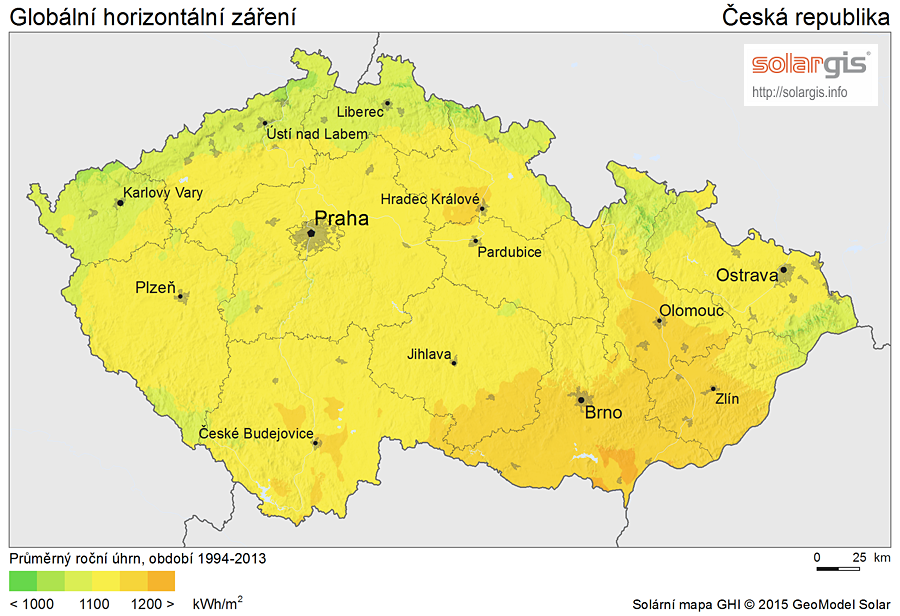
\includegraphics[scale=0.41]{obrazky/Solargis-CZ-GHI.png}
  \end{center}
  \caption{Globální horizontální záření \cite{solargis}}
\end{figure}

\subsubsection*{U solárních panelů se udávají tyto parametry:}
\begin{itemize}
\item Výkon - jaký výkon je panel schopný podávat.
\item Napětí naprázdno - jaké napětí se na svorkách panelu může objevit, pokud
není panel zatížen (spotřebičem).
\item Maximální napětí při plném výkonu - jaké napětí bude na svorkách panelu, pokud
bude zatížen maximálním povoleným proudem.
\item Maximální proud při plném výkonu - maximální povolený odebíraný protékající proud.
\end{itemize}

\subsection*{Akumulátor}
Akumulátor je zařízení, které má schopnost uchovávat energii. Nejběžnější typy elektrických akumulátorů pracují na elektrochemickém principu. Mezi takové akumulátory patří například: nikl-kadmiové (NiCd), nikl-metal hydridový (NiMh), lithium-polymerový (Li-pol), lithium-iontový (Li-ion) a olověný (Pb).

\subsection*{Lithiové akumulátory}
Lithiové akumulátory patří v současnosti k nejpoužívanějším typům akumulátorů. Najdeme je téměř v každé přenosné spotřební elektronice. 
Mezi lithiové akumulátory řadíme lithium-iontové (Li-ion) a novější lithium-polymerové (Li-pol).

Mezi výhody lithiových akumulátorů patří především velká energetická hustota, můžeme tedy mít baterii s vysokou kapacitou s relativně malou hmotností a objemem. Další výhodou je nízké samovybíjení, schopnost dodávat vysoké proudy a také relativně dlouhá životnost.

Mezi nevýhody zmiňme nutnost složitějšího obvodu pro nabíjení. Je nutné hlídat akumulátor před přílišným nabitím a vybitím a také před vysokou teplotou. Je zde také nebezpečí vznícení nebo výbuchu při zkratu.

\subsection*{Olověné akumulátory}
Olověný akumulátor je typ sekundárního galvanického článku s elektrodami na bázi olova. Elektrolytem je kyselina sírová.

Výhodou je především jednodušší obvodové řešení pro nabíjení a také nižší cena vzhledem ke kapacitě akumulátoru.

Nevýhodou je zejména vyšší hmotnost akumulátoru.

%% Vložení souboru 'text/vysledky' s popisem vysledků práce
%\chapter{Výsledky práce}

\chapter{Návrh aplikace}
\section{Architektura aplikace}

Aplikace běžící na Raspberry Pi je napsána v programovacím jazyce Python verze 3.5. Aplikace se spustí po startu operačního systému a provede inicializaci vlákna pro stahování konfiguračního souboru v daných intervalech, poté provede inicializací vlákna pro upload fotografií.

\subsection*{Vícevláknové zpracování}
Aplikace bude provádět současně několik činností.

Bude nutné nepřetržitě monitorovat pohyb, odesílat fotografie a současně vyčítat stav baterie. Také je důležité kontrolovat, zda nedošlo ke změně konfigurace. Z toho důvodu bude třeba program rozdělit do více na sobě nezávislých vláken.

\begin{figure}[h]
  \begin{center}
    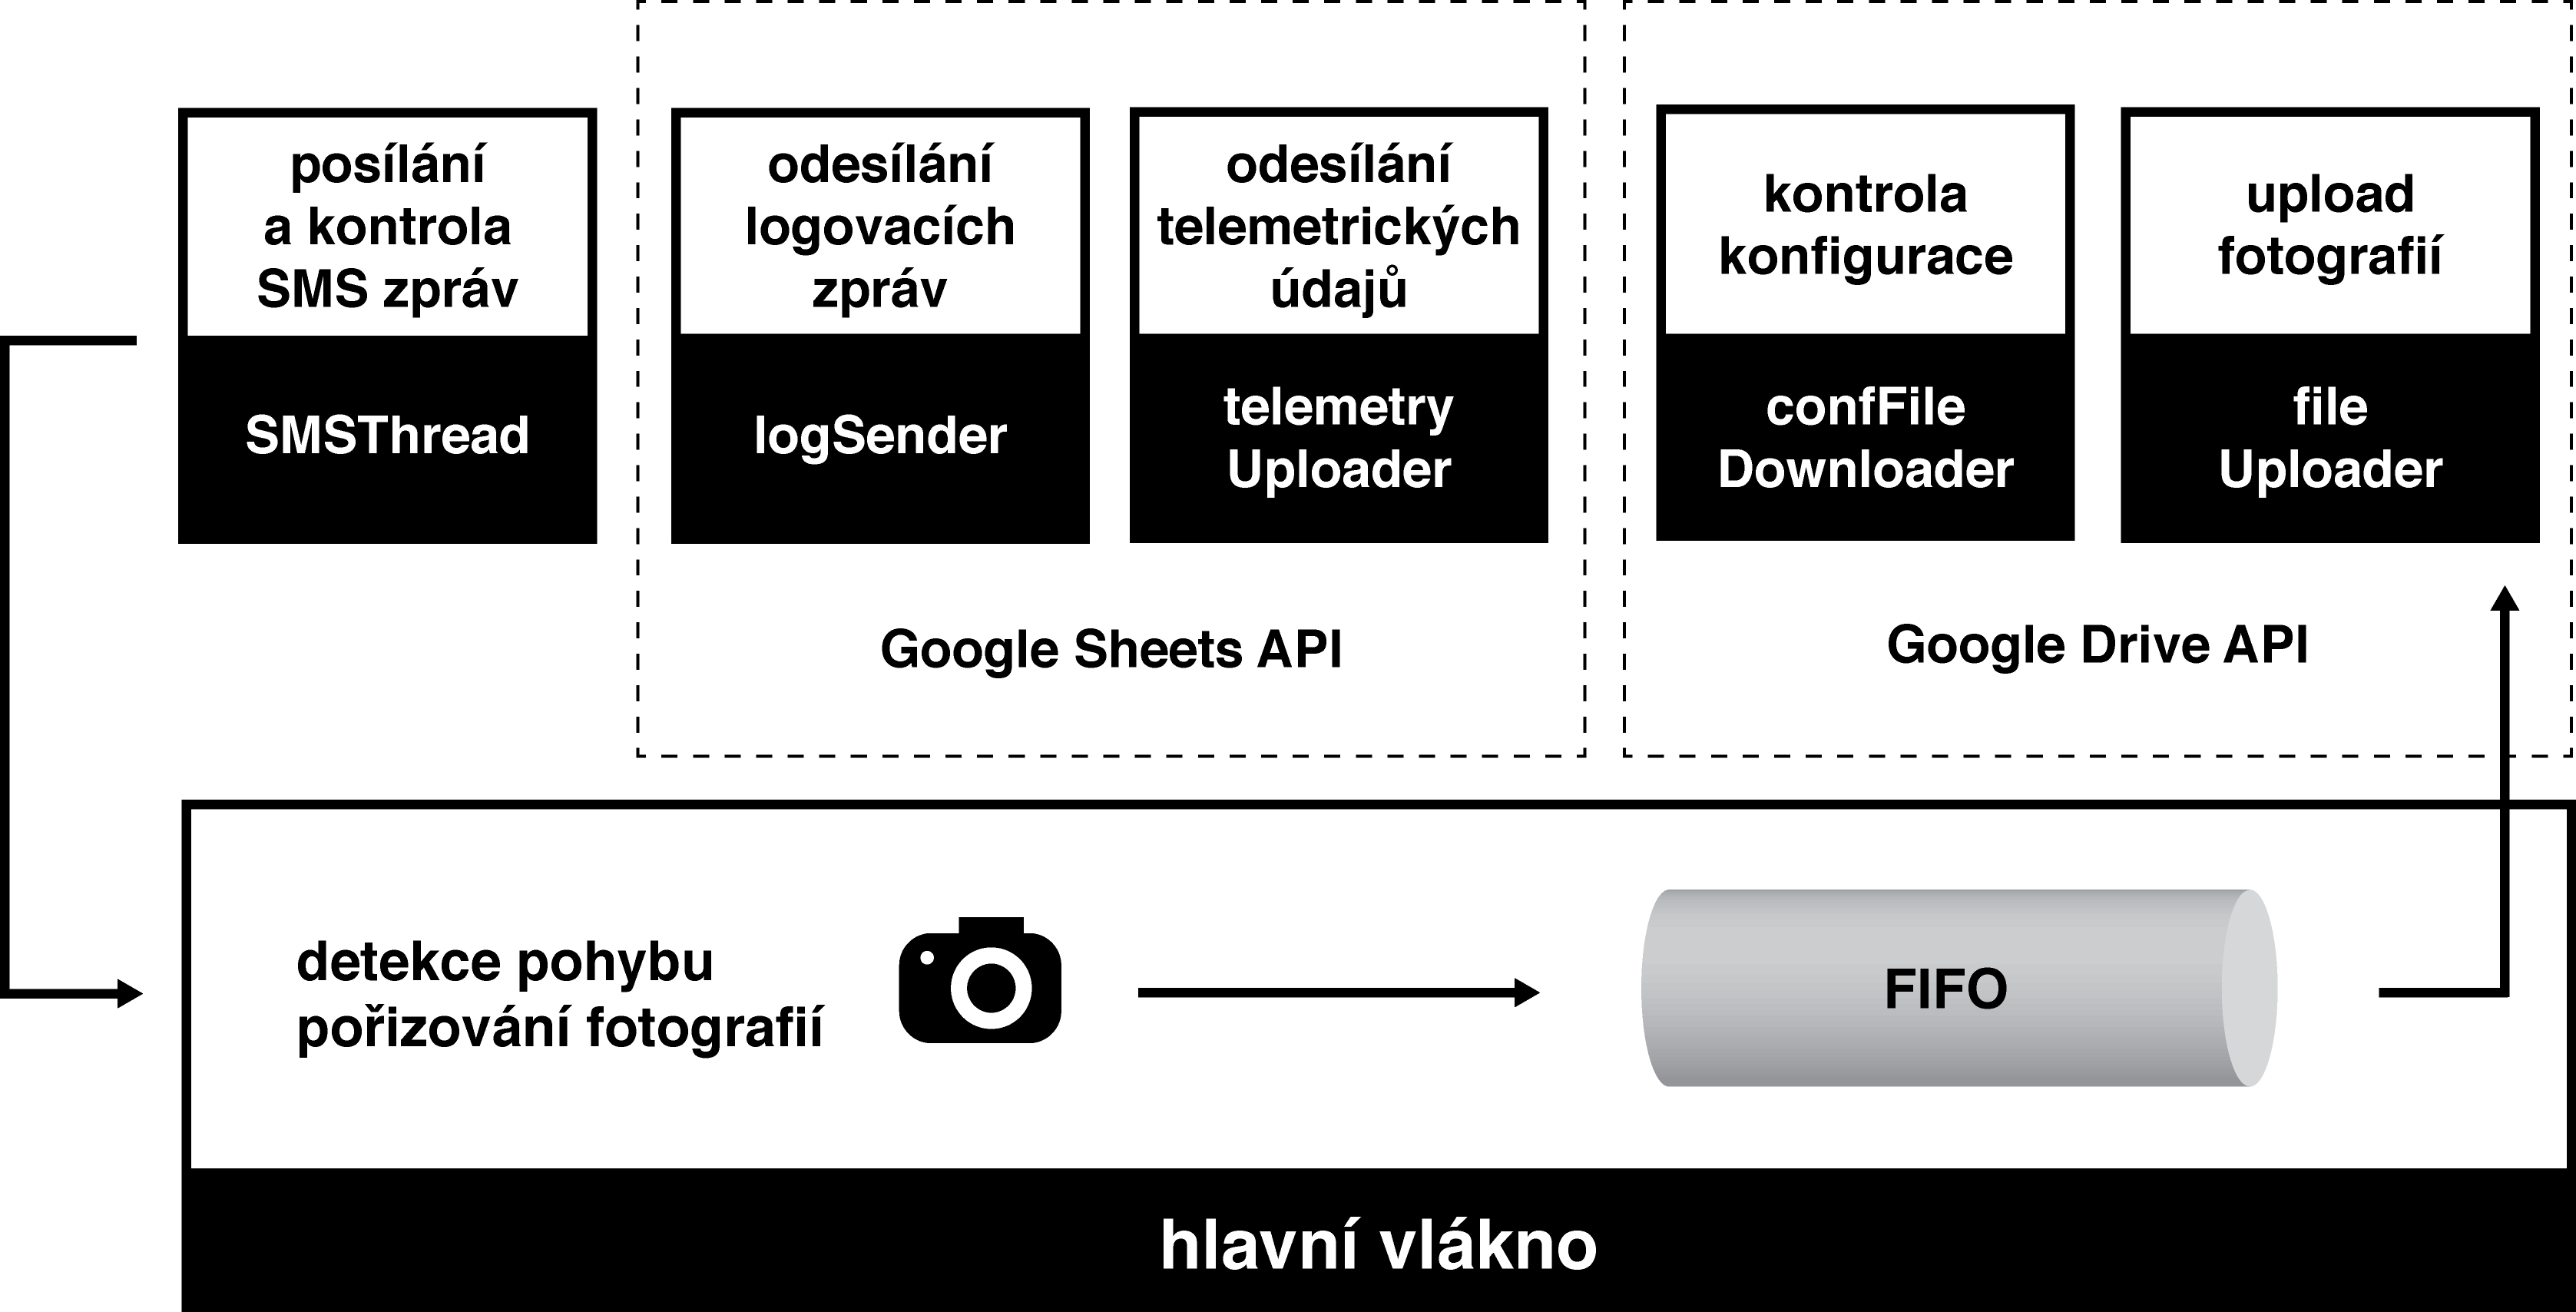
\includegraphics[scale=0.5]{obrazky/schema_aplikace.png}
  \end{center}
  \caption{Architektura aplikace}
\end{figure}

\subsection*{Hlavní vlákno aplikace}
Hlavní vlákno aplikace se stará o detekci pohybu a pořizování fotografií.

Jakmile je detekován pohyb, je provedena zkušební fotografie, ze které je odečtena celková jasová složka snímaného obrazu.

Pokud je hodnota jasu pod prahem denního snímání, jsou nastaveny parametry kamery pro noční režim a je pořízena fotografie.

 Fotografie je zkomprimována, uložena na SD kartu a vložena do fronty pro zaslání do externího úložiště.
 
 Pokud je aktivovaný režim echo, je provedeno ještě dalších 10 fotografií v sekundových intervalech.

\subsection*{Odesílání fotografií do úložiště}
Odesílání fotografií je řešeno ve vlákně nazvaném fileUploader.

Toto vlákno umožňuje autentizaci s Google Drive pomocí OAuth 2.0. Následně je vyčítána fronta a fotografie jsou postupně odesílány do úložiště.

Pokud je aplikace v režimu batch, je odesílání fotografií aktivováno až ve stanovenou dobu.

\subsection*{Kontrola konfigurace}
Vlákno kontroly a stahování konfiguračního souboru zvané confFileDownloader rovněž používá Google Drive API.

Po spuštění vlákna se inicializuje spojení s Google Drive a stáhne se JSON konfigurační soubor podle zadaného identifikátoru. JSON data v konfiguračním souboru jsou přečtena pomocí modulu JSON a naimportována do třídy UserConfig.

V rámci aplikace jsou konfigurační data uložena v modulu config ve třídách BaseConfig a UserConfig, přičemž třídu BaseConfig nelze konfigurovat pomocí JSON a třída UserConfig je určena pro uživatelskou konfiguraci.

Stahování konfiguračního souboru a kontrola změny probíhá ve stanovených intervalech, výchozí hodnota je každých 5 sekund. Pokud vlákno nepracuje, je uspáno.

\subsection*{Odesílání telemetrických údajů}
Vlákno odesílání telemetrických údajů využívá Google Sheets API ke komunikaci s Google Sheets.

Vlákno vyčítá informace o stavu nabíjení akumulátoru ze solárního regulátoru a také informace o využití systémových prostředků jako vytížení CPU a využití operační paměti.

Data se převádí do podoby, kterou je možné vložit do tabulky Google Sheets. Vyčítání dat a odesílání do tabulky je prováděno každých 5 sekund.

\subsection*{Odesílání logovacích zpráv}
Vlákno odesílání logovacích zpráv využívá Google Sheets API ke komunikaci s Google Sheets. 

Vlákno je implementováno jako takzvaný handler pro modul logging, který je využíván pro logování zpráv. Namísto ukládání logovacích zpráv do souboru se zprávy ukládají do fronty a v daných intervalech jsou poslány do listu Google Sheets. 

\subsection*{Odesílání a kontrola SMS zpráv}
Vlákno SMSThread provádí kontrolu přijatých zpráv.

Pokud je přijata SMS zpráva s významem z autorizovaného čísla, tak se provede akce. Pokud je přijata zpráva z neautorizovaného čísla, tak je okamžitě vymazána.

\section{Detekce pohybu}

Zařízení umožňuje dvě metody detekce pohybu - detekce pohybu z obrazu a detekce pohybu pomocí PIR čidla.

Ve výchozím nastavení jsou zapnuty obě metody detekce, avšak detekci pohybu pomocí PIR senzoru je možné vypnout.  

Detekční úhel je dán omezením horizontálního pozorovacího úhlu zvolené kamery. V našem případě výrobce kamery udává pozorovací úhel 62 úhlových stupňů v horizontálním směru a 48 úhlových stupňů ve vertikálním směru.

\subsection*{Detekce pohybu pomocí PIR}
Výhodou detekce pohybu pomocí PIR senzoru je nezávislost na osvětlení scény. Je možné ji použít například v noci, kdy již nelze použít detekci pohybu z obrazu z důvodu necitlivosti kamery.

Další výhodou detekce pohybu PIR senzorem je nízká výpočetní náročnost, protože je kontrolována pouze jedna logická hodnota. 

Efektivita detekce pohybu PIR senzorem je dána těmito parametry: citlivosti PIR senzoru, pozorovacím úhlem kamery a dosahem LED přísvitu.

PIR senzor použitý v této práci má udávanou spolehlivou detekční vzdálenost maximálně 5 metrů, z čehož vyplývá dosah LED přísvitu, tedy také 5 metrů.

\subsection*{Detekce pohybu z obrazu}
Výhodou detekce pohybu z obrazu je kupříkladu možnost umístit kameru za sklo, respektive okno. V případě detekce pohybu pomocí PIR senzoru toto není možné.

Detekce pohybu z obrazu využívá algoritmus výpočtu vektorů pohybu z optického toku.

Tato softwarová metoda je výpočetně velmi náročná, ale patří mezi nejspolehlivější metody. Není tolik ovlivňována změnou osvětlení na snímané scéně a je odolná proti šumu.

V případě Raspberry Pi je kodér H.264 implementován přímo na GPU. Tento princip se využívá například v kodéru MPEG pro kompresi videa.

\subsection*{Hledání vektorů pohybu}
Data o vektorech pohybu je možné získat přímo z kodéru H.264.

V našem případě snímáme video v rozlišením 640x368 pixelů. Vektory pohybu jsou počítány přímo na úrovni makrobloků (makroblok má rozměry 16x16 pixelů).

V našem případě bude tedy mít matice vektorů pohybu rozměry 40+1 sloupců a 23 řádků. Matice obsahuje jeden sloupec dat navíc.

Data o pohybu mají velikost 4 bajty. Každá z proměnných vektoru pohybu [x] a [y] má velikost jeden bajt, zbývající dva bajty obsahují sumu absolutních diferencí (SAD). 

Suma absolutních diferencí udává míru odlišnosti mezi referenčním blokem a současným blokem. Je vypočtena jako suma rozdílů absolutních hodnot mezi jednotlivými pixely v původním bloku a bloku, který porovnáváme. 

\begin{figure}[h]
  \begin{center}
    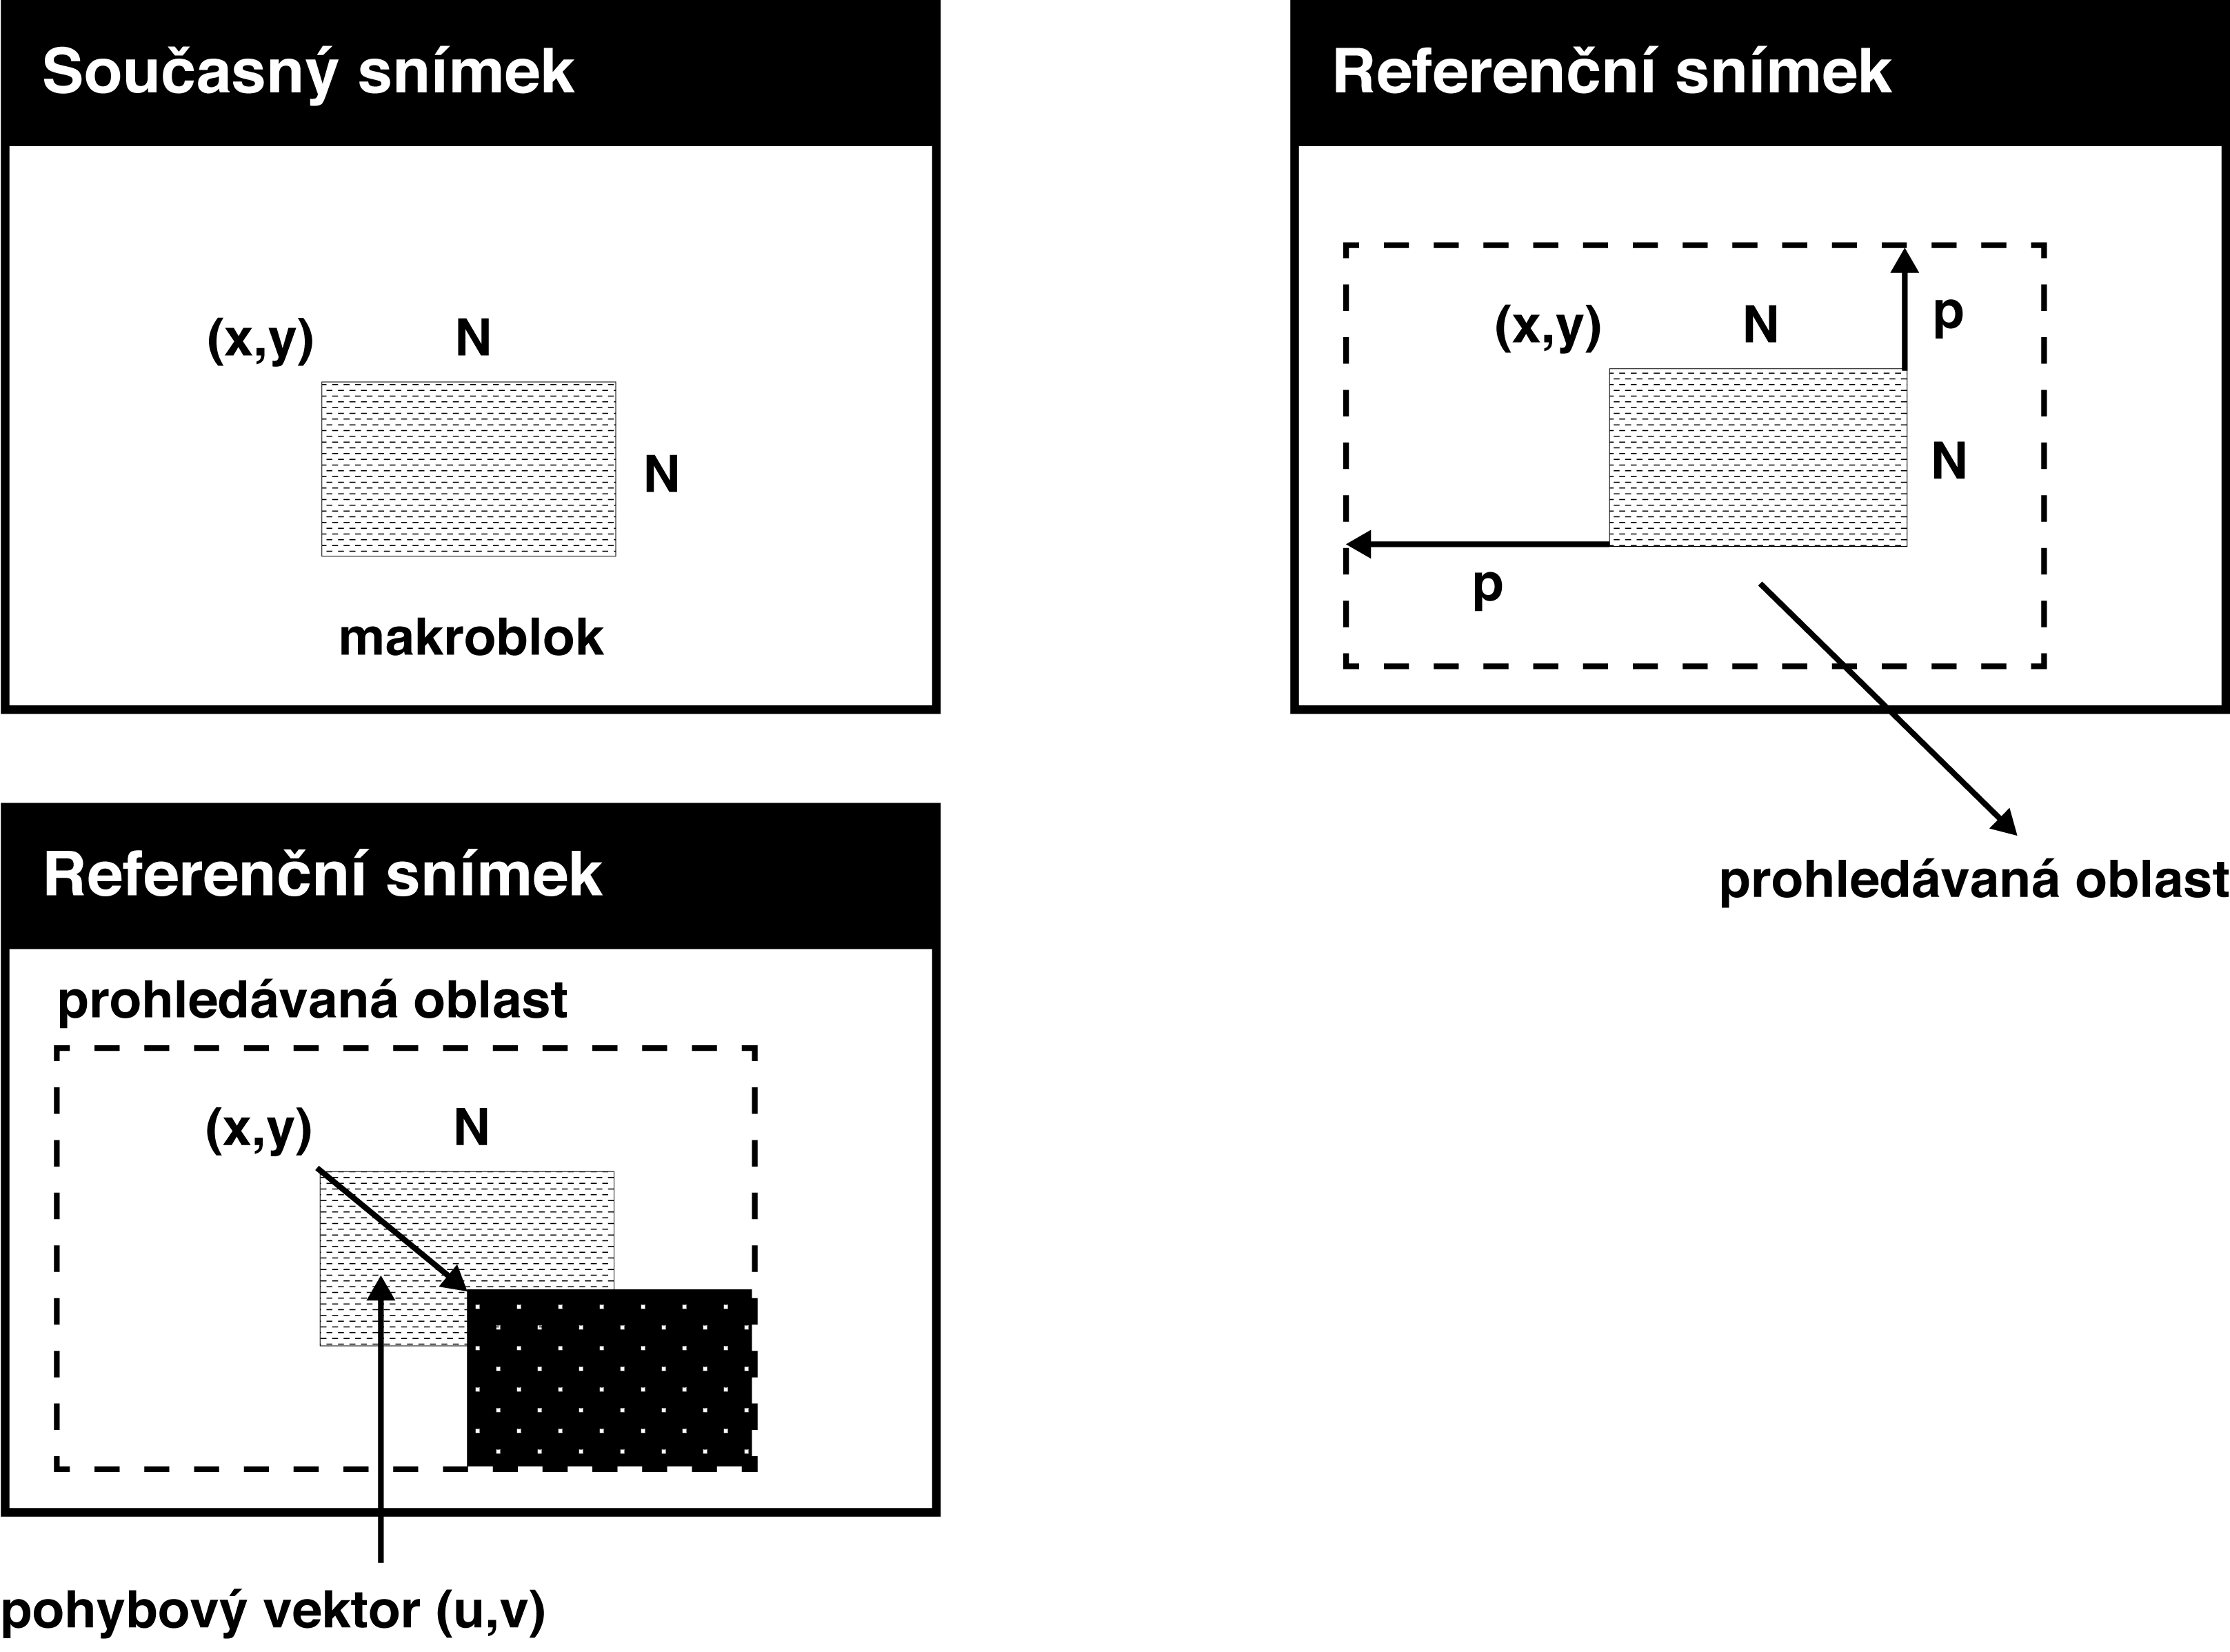
\includegraphics[scale=0.5]{obrazky/makroblok.png}
  \end{center}
  \caption{Hledání vektorů pohybu}
\end{figure}

\subsection*{Třída pro detekci pohybu z obrazu}

PiMotionAnalysis je třída poskytnutá knihovnou PiCamera pro detekci pohybu z obrazu v reálném čase, využívající metodu počítání vektorů pohybu.

Třída implementuje metodu analyse, která je volána pro každý snímek. V této metodě je nutné implementovat logiku počítání velikosti vektorů a prahování.

Práh detekce je možné parametrizovat minimální velikostí vektoru, tj. o kolik se daný makroblok posunul. A také počtem vektorů splňující danou minimální velikost.

Níže je ukázka výpočtu velikosti pohybových vektorů za použití modulu Numpy.

\begin{minted}[breaklines,frame=single]{python}
class vectorMotionAnalysis(picamera.array.PiMotionAnalysis):
    def analyse(self, a):
        a = np.sqrt(
            np.square(a['x'].astype(np.float)) +
            np.square(a['y'].astype(np.float))
            ).clip(0, 255).astype(np.uint8)
        # Jestli je více jak 10 vektorů s velikostí 
        # větší než 60, pohyb je detekován
        if (a > 60).sum() > 10:
            print('Pohyb detekován!')
\end{minted}

\section{Řízení snímání fotografií}
Řízení snímání fotografií je poskytnuto třídou CaptureHandler a metodou tick.

Metoda tick je volána každou sekundu.

Pokud je zavolána metoda motion\_detected a přitom současně není zpracovávána žádná jiná fotografie, provede se metoda tick.

\subsection*{Parametry snímaných fotografií}
Ve výchozím nastavení se snímá v rozlišením 640x368 pixelů.

Pro denní režim je nastavení módu expozice a vyvážení bílé automatické. Rychlost uzávěrky je také automatická. V nočním režimu je použit expoziční režim nightpreview a doba uzávěrky je nastavena na 200 ms.

Fotografie jsou zkomprimovány a optimalizovány za použití modulu PIL ve výchozím nastavením komprese 75.
\clearpage
\begin{minted}[frame=single]{python}
# Ukázka snímání fotografie v noci 
with picamera.PiCamera() as camera:
    camera.resolution = (1280, 720)
    # Snímkovací frekvence je nastavena na 1 fps 
    # Doba uzávěrky je nastavena na 200 milisekund a ISO na 800
    camera.framerate = 1
    camera.shutter_speed = 200000
    camera.exposure_mode = 'nightpreview'
    camera.iso = 800
    # Kamera potřebuje čas na změření AWB - Auto white balance
    sleep(10)
    camera.capture('dark.jpg')
    # Snímek je pořízen
\end{minted}

\subsection*{Detekci denní doby}
Detekce intenzity osvětlení (respektive denní doby) je řešena softwarově.

Využívá se výpočtu průměrné hodnoty pixelů vyjádřené v RGB.

Tato metoda není příliš přesná, ale je dostačující pro rozhodnutí, zda-li má být fotografie pořízena v nočním režimu s přísvitem.

Měří se průměrná hodnota pixelu v testované matici.

Experimentálně bylo zjištěno, že pokud je průměrná hodnota vyšší jak 100, můžeme prohlásit, že světelné podmínky jsou dostatečné pro použití parametrů pro denní snímání.

\begin{minted}[breaklines,frame=single]{python}
def scanIfDay():
    with picamera.PiCamera() as camera:
        camera.resolution = (testWidth, testHeight)
        with picamera.array.PiRGBArray(camera) as stream:
            camera.exposure_mode = 'auto'
            camera.awb_mode = 'auto'
            camera.capture(stream, format='rgb')
            pixAverage = int(np.average(stream.array[...,1]))
    logging.info("Light Meter pixAverage=%i" % pixAverage)
    if (pixAverage > 100):
        return True
    else:
        return False
\end{minted}




\subsection*{Vývojový diagram detekce pohybu}

\usetikzlibrary{positioning, shapes.geometric, arrows}

\tikzstyle{startstop} = [rectangle, rounded corners, minimum width=3cm, minimum height=1cm,text centered, draw=black]
\tikzstyle{io} = [trapezium, trapezium left angle=70, trapezium right angle=110, minimum width=3cm, minimum height=1cm, text centered, draw=black]
\tikzstyle{process} = [rectangle, minimum width=3cm, minimum height=1cm, text centered, text width=3cm, draw=black]
\tikzstyle{decision} = [diamond, minimum width=3cm, minimum height=1cm, text centered, text width=3cm, draw=black]
\tikzstyle{arrow} = [thick,->,>=stealth]
\begin{tikzpicture}[node distance=2.5cm]

%Nodes
\node (start) [startstop] {Start};
%\node (in1) [process, below of=start] {Načtení %konfiguračního souboru JSON};
\node (promod) [process, below of=start] {Volba módu};
\node (dec1) [decision, below of=promod, yshift=-0.5cm] {Je noc?};
\node (pro1a) [process, below of=dec1, yshift=-1cm] {Denní snímání};
\node (pro1b) [process, right of=dec1, xshift=3cm] {Noční snímání};
\node (pro2) [process, below of=pro1a] {Pořízení fotografie};
\node (pro3) [io, below of=pro2] {Zkomprimovat a uložit na SD kartu};
\node (out1) [io, below of=pro3] {Vložení fotografie do fronty na upload};
\node (stop) [startstop, below of=out1] {Stop};

%Arrows
%\draw [arrow] (start) -- (in1);
%\draw [arrow] (in1) -- (promod);
\draw [arrow] (start) -- (promod);
\draw [arrow] (promod) -- (dec1);
\draw [arrow] (dec1) -- node[anchor=east] {False} (pro1a);
\draw [arrow] (dec1) -- node[anchor=south] {True} (pro1b);
\draw [arrow] (pro1b) -- (pro2);
\draw [arrow] (pro1a) -- (pro2);
\draw [arrow] (pro2) -- (pro3);
\draw [arrow] (pro3) -- (out1);
\draw [arrow] (out1) -- (stop);

\end{tikzpicture}



\clearpage
\section{Detekce pohybu z PIR pomocí obsluhy přerušení}
Ukázka řešení detekce pohybu ze senzoru PIR pomocí obsluhy přerušení.

Obsluha přerušení je řešena pomocí modulu GPIO.

PIR senzor je připojen k GPIO pinu 7.

\begin{minted}[breaklines,frame=single]{python}
import RPi.GPIO as GPIO
import time

GPIO.setmode(GPIO.BCM)  # nastav mod cislovani na BCM
PIR_PIN = 7             # nastaveni PIR na pin 7 (BCM)
GPIO.setup(PIR_PIN, GPIO.IN) # nastavime pin na vstupni

def MOTION(PIR_PIN):
    print("Detekovan pohyb!")

print ("Test PIR senzoru") # pockame na inicializaci
time.sleep(2)
print("Pripraven")

try:
    GPIO.add_event_detect(PIR_PIN, GPIO.RISING, callback=MOTION) 

while 1:
    time.sleep(100)

except KeyboardInterrupt:
    print("Konec") # ukonceni na preruseni z klavesnice
    GPIO.cleanup()

\end{minted}

\clearpage

\section*{Odesílání fotografií na cloudové úložiště}
Po nasnímání jsou fotografie zkomprimovány a optimalizovány s použitím JPEG podle nastavené úrovně komprese a uloženy na lokální úložiště.

Jméno fotografie je časová známka v době, kdy byla pořízena.

Toto jméno souboru fotografie je následně vloženo do fronty, která je sdílena s vláknem pro odesílání fotografií, ve kterém je v daných časových intervalech vyčítána a nezávisle na běhu hlavního vlákna je posílána do vzdáleného úložiště.

\section{Ovládání aplikace}

\subsection*{Ovládací panel aplikace}

Ovládací panel je řešen prostřednictvím aplikace Google Sheets pomocí Google API, která umožňuje integraci aplikací napsaných v jazyce Python s produkty Google.

K tomuto řešení bylo přistoupeno z důvodu požadavku na vzdálenou konfiguraci aplikace bez nutnosti provozovat nějaký webový server pro běh rozhraní.

Google API je tzv. REST, to znamená, že je implementováno na protokolu HTTP.

Z toho plynoucí výhody jsou jednoduchost implementace a malý přenášený objem dat. Jsou přenášena pouze ta data, která jsou vyžádána.

V neposlední řadě je to také spolehlivost a rychlost zajištěná servery Google a také možnost publikace celého dokumentu veřejně přístupnou HTML stránkou. 

Rozhraní vytvořené pro aplikaci obsahuje pět sešitů.

Úvodní sešit nazvaný Dashboard obsahuje grafické shrnutí údajů o stavu nabíjení a napájení a také o stavu systémových prostředků jako je vytížení CPU a RAM.

Data, ze kterých se vychází, se ukládají do sešitu zvaném Log.

V dalším sešitu jsou zobrazeny náhledy fotografií nasnímaných při detekci pohybu.

Následující sešit obsahuje log zpráv, označených jmény vláken, odkud zprávy přišly.

Zprávy jsou řazeny do čtyř kategorií:
\begin{itemize}
    \item DEBUG - podrobné informace o chodu programu, je možné je vypnout. 
    \item INFO - informační zprávy.
    \item WARNING - varování neohrožující chod programu.
    \item ERROR - chyby.
    \item CRITICAL - velmi závážné chyby, které znemožňují chod programu.
\end{itemize}

Poslední sešit umožňuje konfigurovat zařízení pomocí dialogového okna s formulářem.

Na základě zadaných dat je vygenerován konfigurační soubor ve formátu JSON, který je poté stažen ve vlákně pro kontrolu konfigurace.

\begin{figure}[h]
  \begin{center}
    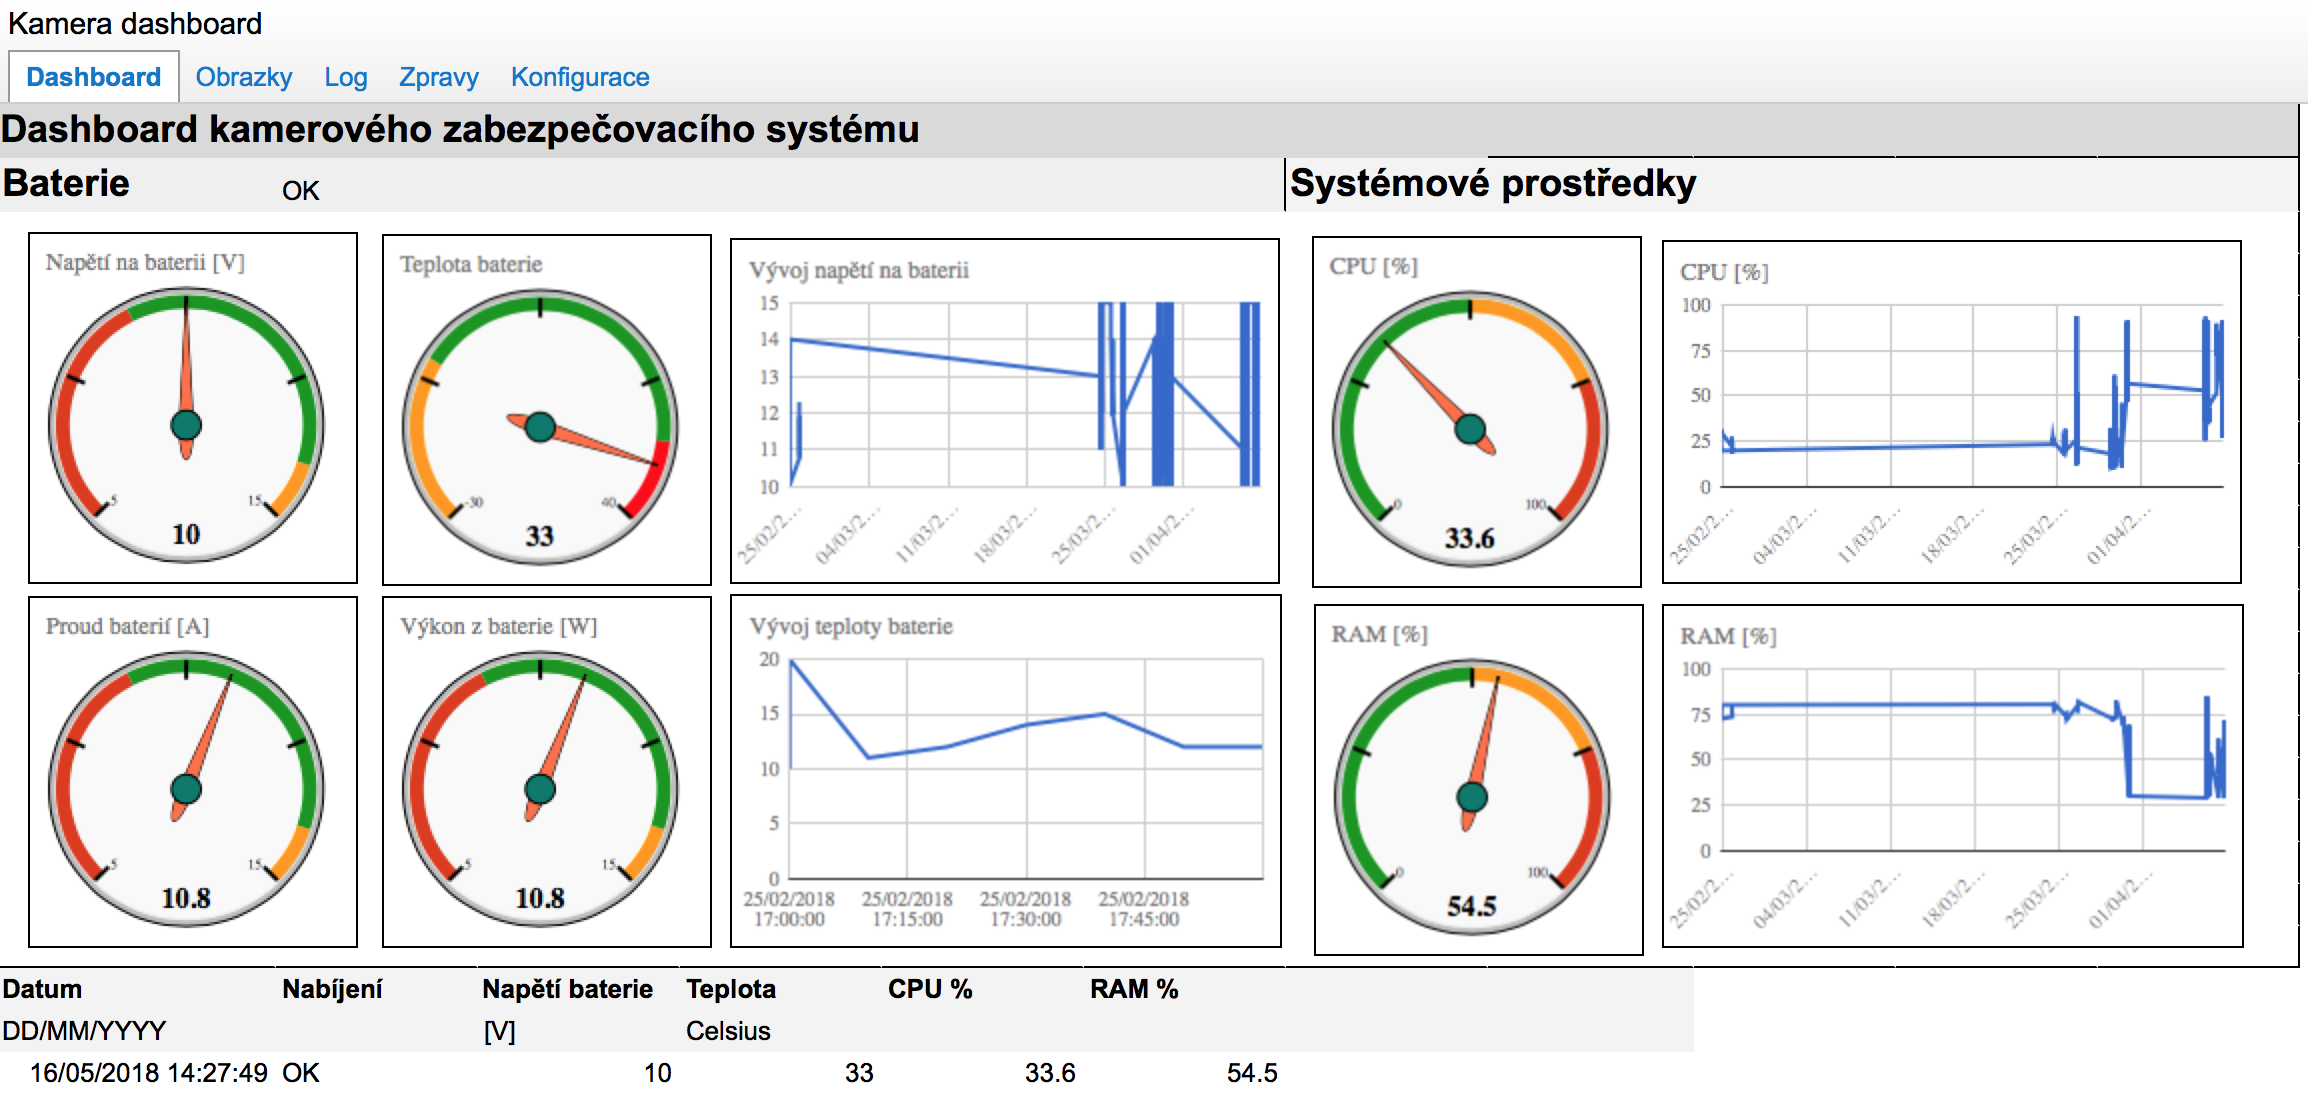
\includegraphics[scale=0.3]{obrazky/dashboard2.png}
  \end{center}
  \caption{Informační panel aplikace}
\end{figure}

\begin{figure}[h]
  \begin{center}
    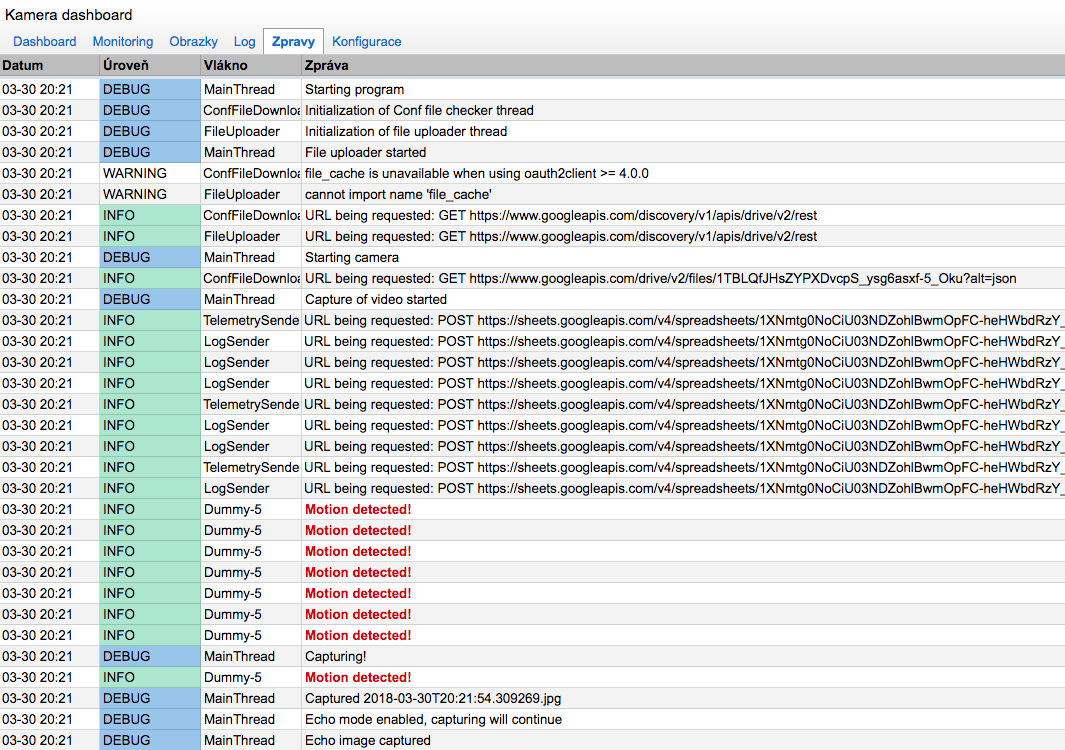
\includegraphics[scale=0.35]{obrazky/logy.png}
  \end{center}
  \caption{Panel aplikace obsahující log}
\end{figure}

\subsection*{Ovládání a notifikace pomocí SMS}

Aplikaci je možné ovládat pomocí SMS z jednoho autorizovaného čísla, pokud je v konfiguračním souboru nastavený parametr SMS control.


\begin{table}[h]
\centering
\caption{Příkazy SMS}
\label{sms}
\begin{tabular}{|l|l|l|}
\hline
\textbf{SMS příkaz} & \textbf{Popis}            & \textbf{Odpověď} \\ \hline
BATTERY             & Informace o stavu baterie & Charging 12.3V     \\ \hline
TAKEPHOTO           & Okamžitá fotografie       &   -               \\ \hline
SET MODE <x>          & Nastav mód na x           & Mode has been set to <x>     \\ \hline
Q MODE              & Dotaz na aktivní mód      & Current mode is <x>     \\ \hline
 -                   & Nesprávný příkaz     &   Command not recognized                \\ \hline

\end{tabular}
\end{table}

\subsection*{Notifikace pomocí emailu}

Upozornění na detekci pohybu je také odesláno e-mailem prostřednictvím Google Cloud.

Kontrola nových fotografií na Google Drive je spouštěna každou minutu.

Pokud jsou detekovány nové fotografie, tak je odeslán e-mail na zvolenou e-mailovou adresu spolu s fotografiemi, které byly pořízeny. Následně se aktualizuje seznam fotografií v sešitu.


\section{Konfigurace}

Konfigurační data jsou v rámci aplikace uloženy ve dvou třídách - BaseConfig a UserConfig. Vzdáleně měnit je možné pouze konfigurace třídy UserConfig.

Konfigurace je načítána ze souboru ve formátu JSON, který je umístěn na úložišti Google Drive. Po stažení je zahájena kontrola a parsování souboru do třídy UserConfig.

Konfigurační soubor je v určitých intervalech dotazován na změnu. Pokud byl konfigurační soubor změněn, je stažen a načten. Toto je řešeno ve vlákně ConfFileDownloader.

\subsection*{Režim detekce}
Aplikace pracuje ve čtyřech základních režimech.
\begin{itemize}
    \item Real-time
    \item Batch
    \item On-demand
    \item Interval
\end{itemize}

\subsection*{Real-time režim}
V tomto režimu se fotografie pořídí ihned, jakmile je detekován pohyb.

Fotografie je také ihned odeslána na úložiště. Volitelně je pak možné zapnout upozornění SMS zprávou na zadané telefonní číslo a tzv. „dozvuk“, kdy se bude pokračovat ve snímkování každou sekundu i po prvotní detekci pohybu po následujících deset sekund.

Režim má v JSON konfiguračním souboru pod paremetrem \textit{mode} přiřazenou hodnotu \textit{realtime}.

\subsection*{Batch režim}
Tento režim funguje obdobně jako režim Real-time. Snímky však nejsou odeslány ihned po detekci pohybu, ale pouze jednou denně ve zvolené době.

Volitelně je pak možné zapnout upozornění SMS zprávou na zadané telefonní číslo a tzv.  „dozvuk“, kdy se bude pokračovat ve snímkování i po detekci pohybu v zadaném intervalu.

Režim má v JSON konfiguračním souboru pod paremetrem \textit{mode} přiřazenou hodnotu \textit{batch}.

\subsection*{On-demand}
On-demand, neboli na vyžádání, je režim, kdy se fotografie pořídí pouze na vyžádání pomocí SMS zprávy.

Režim má v JSON konfiguračním souboru pod paremetrem \textit{mode} přiřazenou hodnotu \textit{demand}.

\subsection*{Interval}
Tento režim umožňuje nastavení pravidelného snímkování v daném intervalu. Interval se nastavuje v minutách pomocí parametru interval.

Režim má v JSON konfiguračním souboru pod paremetrem \textit{mode} přiřazenou hodnotu \textit{interval}.

\subsection*{Režim echo}
Režim echo je volitelným parametrem pro nastavení „dozvuku“, tj. snímání dalších deseti fotografií po první detekci v sekundových intervalech.

\subsection*{Konfigurační soubor}
Parametrem \textit{mode} se nastavuje pracovní režim detekce, jsou povoleny čtyři hodnoty: \textit{realtime, batch, demand a interval}.

Parametr \textit{echo} je volitelným parametrem pro nastavení  „dozvuku“, tj. snímání fotografií ve stanoveném intervalu po první detekci a uplatňuje se pouze pokud je zvolen režim real-time nebo batch.

Parametr \textit{interval} nastavuje interval snímkování pro režim interval. Je zadáván v sekundách.

Ovládání a notifikace pomocí SMS zpráv je upravena parametry \textit{SMS\_notification}, \textit{SMS\_control} a \textit{authorized\_numbers}. Pole \textit{authorized\_number} obsahuje telefonní číslo, které může ovládat zařízení pomocí SMS příkazů a zároveň dostáví notifikace.

K datovému typu string bylo přistoupeno z důvodu lepší serializace z HTML formulářů.

\begin{table}[h]
\centering
\caption{Parametry konfiguračního souboru}
\label{}
\begin{tabular}{|l|l|l|}
\hline
\textbf{Parametr}  & \textbf{Datový typ} & \textbf{Popis}                 \\ \hline
mode               & string              & Metoda detekce                 \\ \hline
echo               & string             & Použití dozvuku        \\ \hline
interval              & number             & Interval        \\ \hline
SMS\_notification  & string             & Notifikace pomocí SMS          \\ \hline
SMS\_control       & string             & Ovládání pomocí SMS            \\ \hline
authorized\_number & string              & Autorizované číslo              \\ \hline
\end{tabular}
\end{table}

\begin{minted}[frame=single]{json}
{
	"mode": "realtime",
	"echo": "off",
	"interval": 5,
	"use_pir": "on",
	"SMS_notification": "off",
	"SMS_control": "on",
	"authorized_number": "+420733122122"
}
\end{minted}

\clearpage
\subsection*{Rozhraní pro konfiguraci}

Rozhraní pro konfiguraci je poskytnuto jako nadstavba nad Google Sheets vytvořená pomocí HTML a JavaScriptu. Samotná konfigurace se provádí v uživatelsky přívětivém formuláři. Po odeslání se pomocí JavaScriptu serializují data uložena ve formuláři do podoby JSON - JavaScript Object Notation a následně se uloží na Google Drive.

\begin{figure}[h]
  \begin{center}
    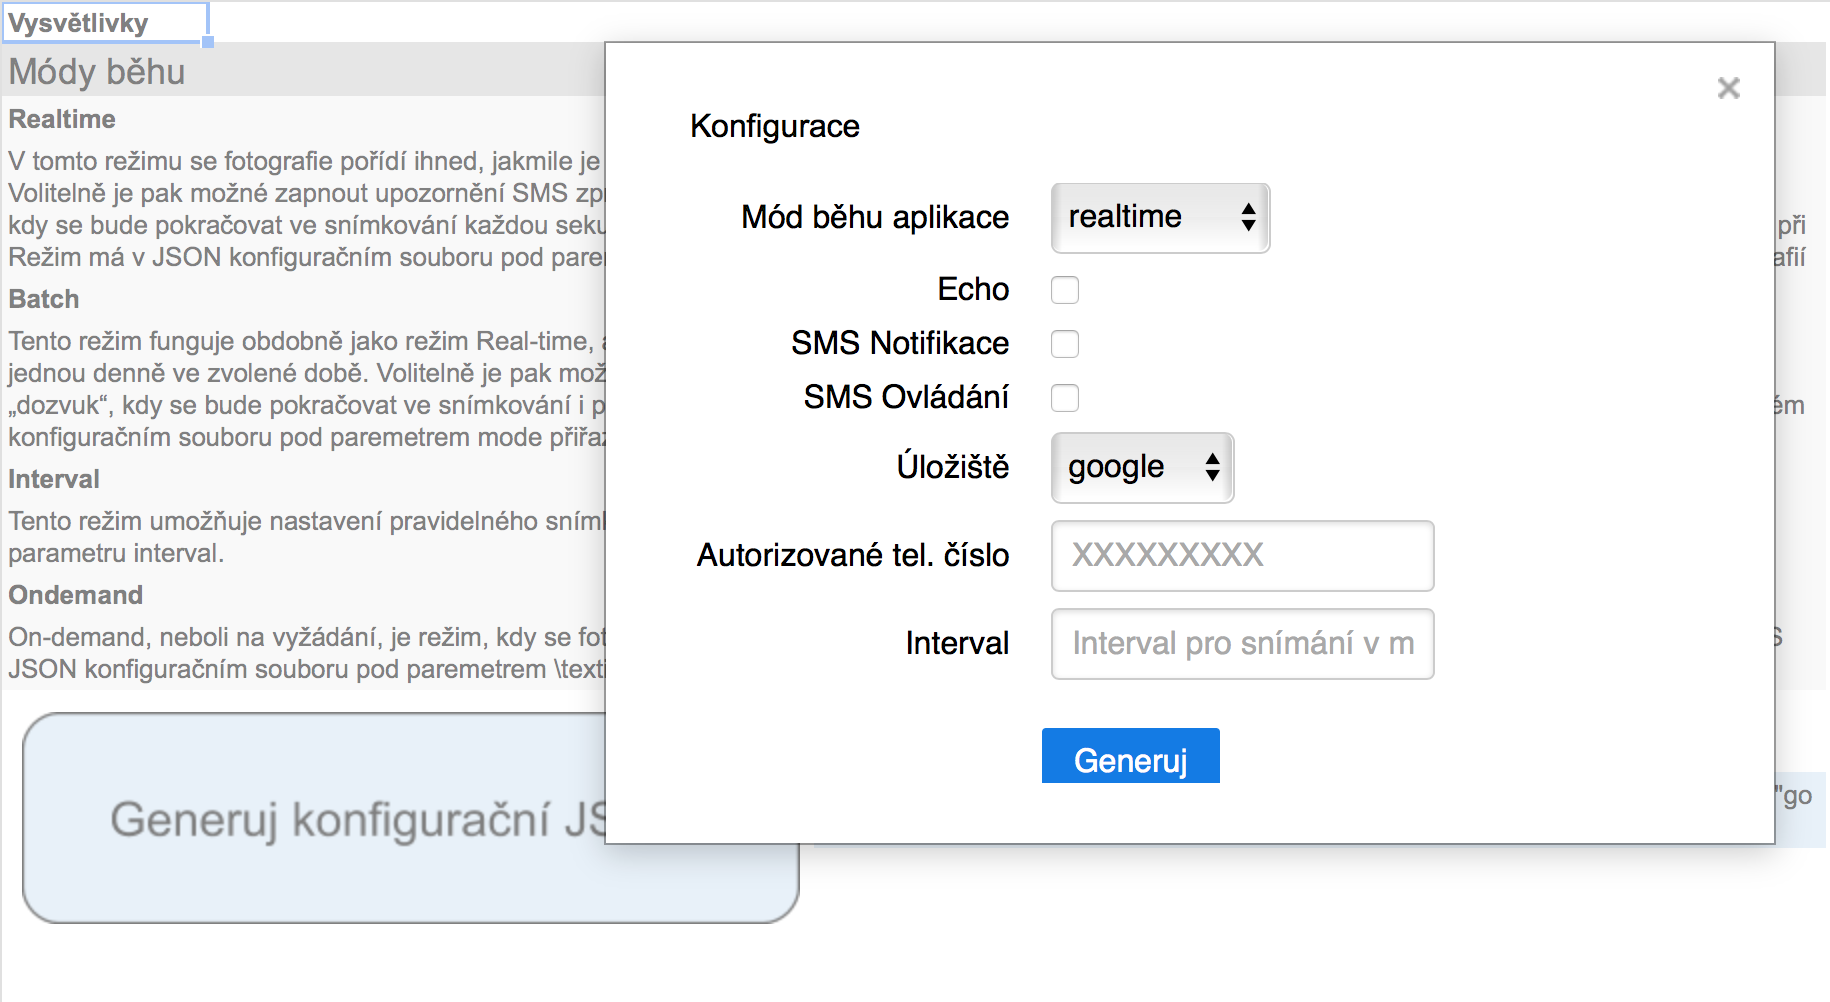
\includegraphics[scale=0.35]{obrazky/konfigurace.png}
  \end{center}
  \caption{Rozhraní pro konfiguraci}
\end{figure}


\section{Sledování stavu baterie}

Vyčítání stavu baterie a průběhu nabíjení ze solárního regulátoru Epsolar LS1024B je možné realizovat pomocí rozšiřujícího modulu epsolar-tracer, který umožňuje vyčítat následující informace: napětí baterie, napětí na solárním panelu, proud na zátěži, nabíjecí proud a teplotu baterie.

Komunikace je realizována pomocí protokolu Modbus.
\clearpage

\chapter{Návrh zapojení}

\section{Prototypování}

Před samotným návrhem výsledného zařízení, je vhodné nejprve komponenty sestavit na nepájivém poli abychom otestovali vzájemnou funkčnost a případně odstranili nedostatky.

\begin{figure}[h]
  \begin{center}
    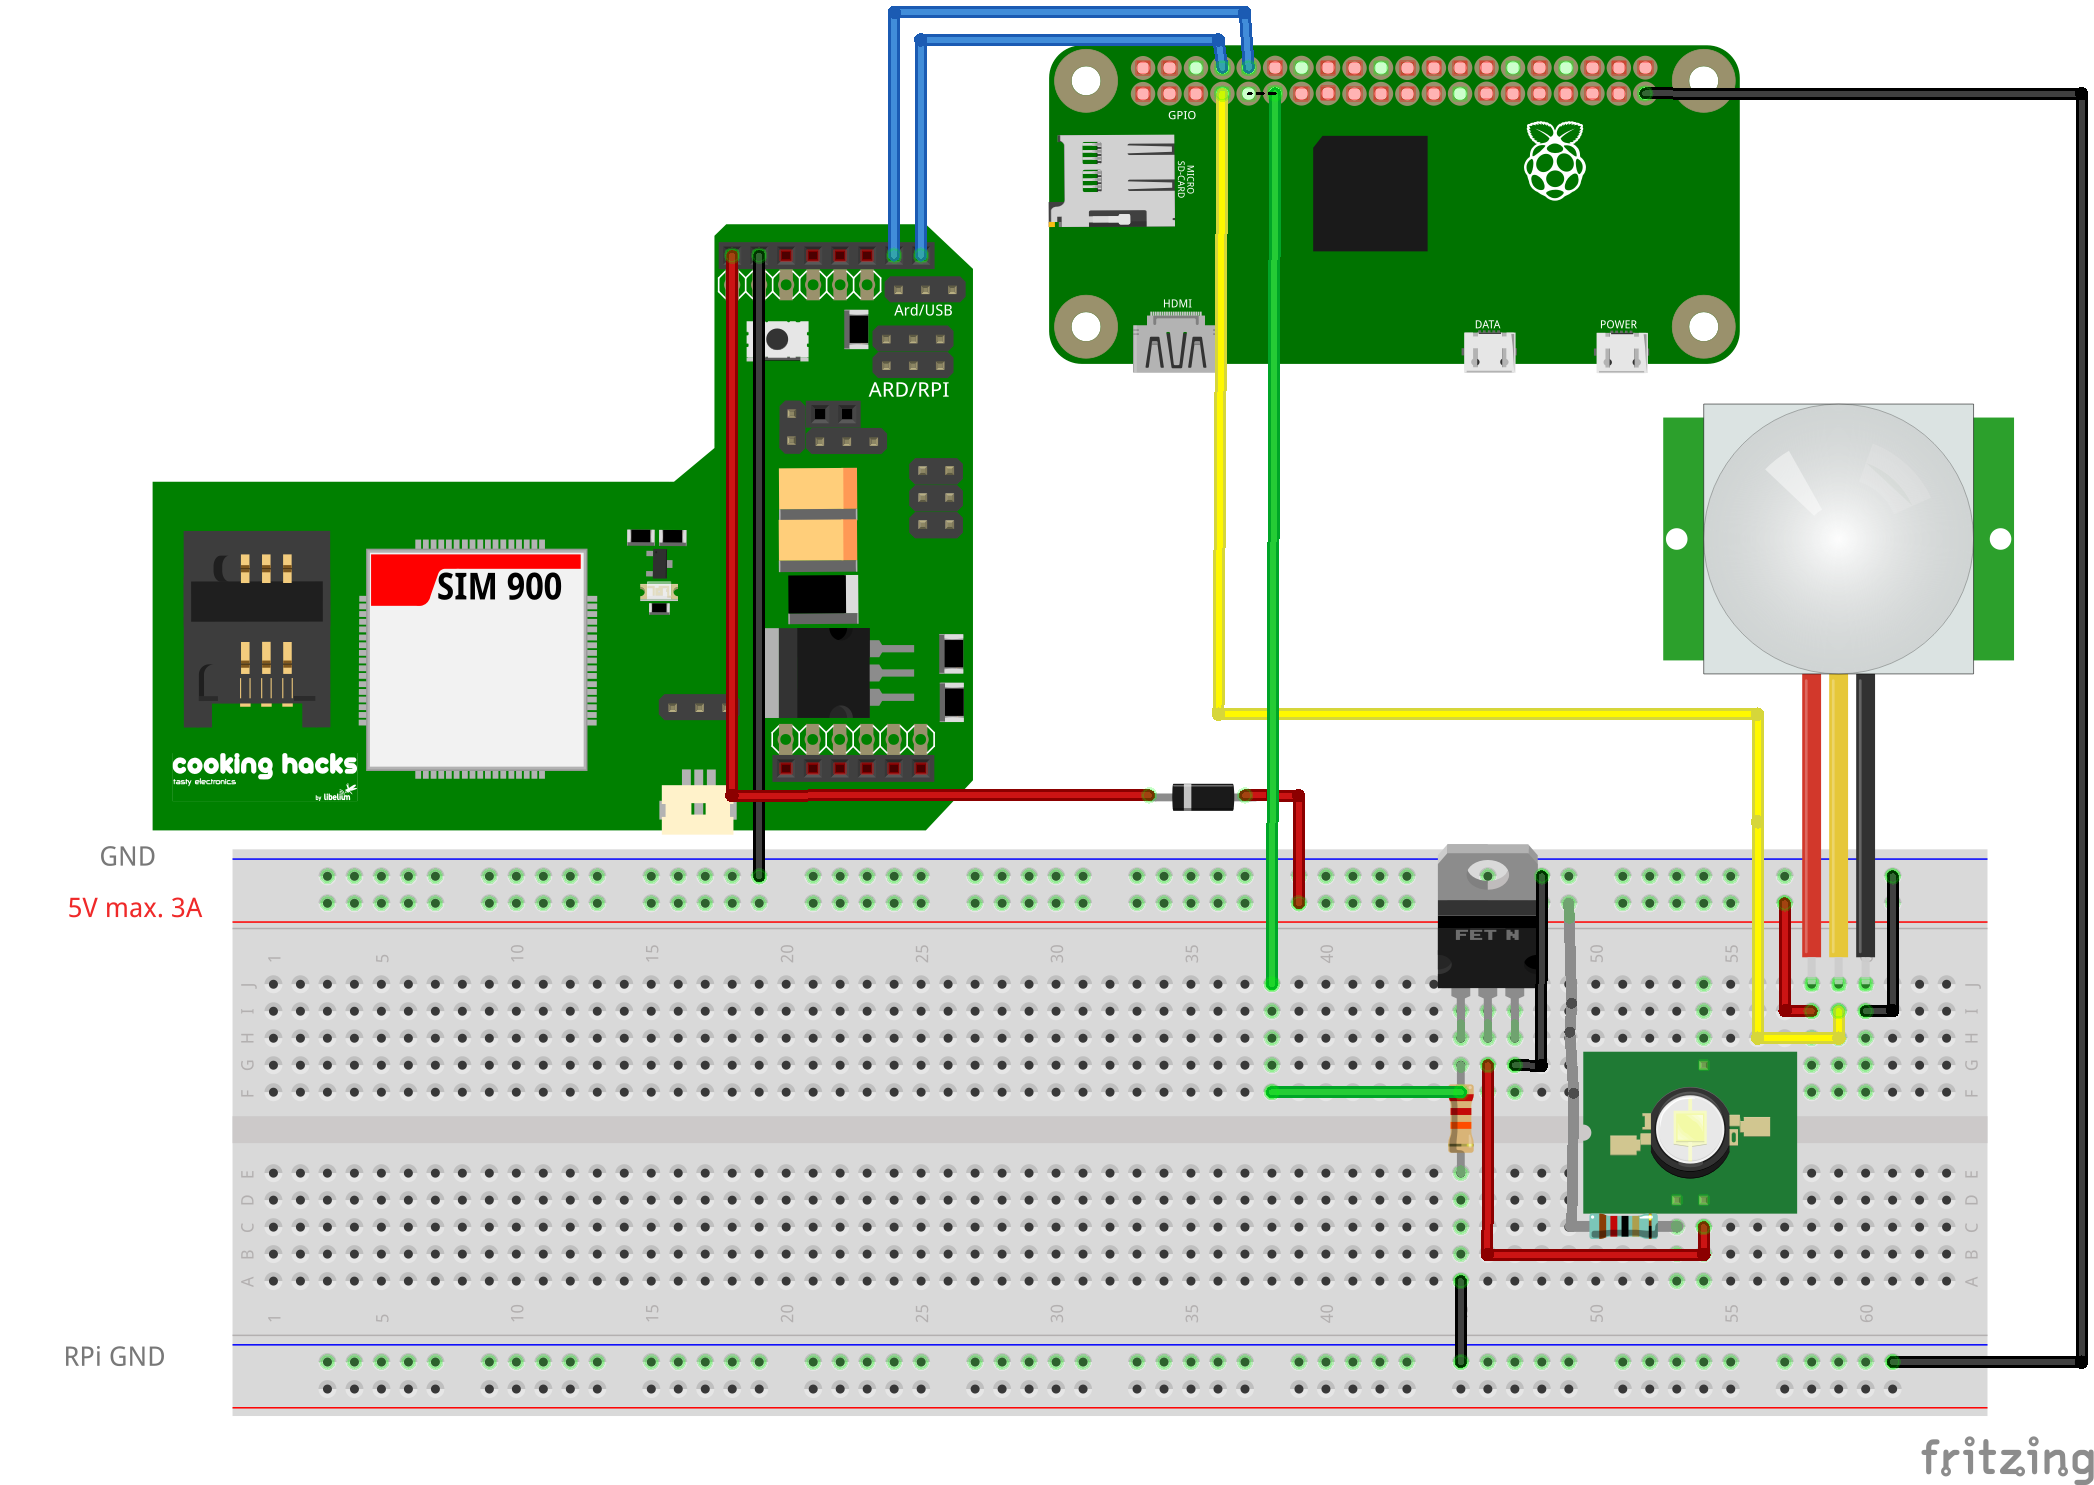
\includegraphics[scale=0.75]{obrazky/schema.png}
  \end{center}
  \caption{Prototyp zařízení sestavený na nepájivém poli}
\end{figure}

\section{Řešení napájení}
\subsubsection{Spotřeba zařízení}
Před samotným návrhem napájecího obvodu je nutné nejprve zjistit proudový odběr jednotlivých komponent zařízení z katalogů.

% Please add the following required packages to your document preamble:
% \usepackage{multirow}
%\begin{table}[]
%\centering
%\caption{My caption}
%\label{my-label}
%\begin{tabular}{|l|l|l|l|}
%\hline
%\multirow{2}{*}{\textbf{Komponenta}} & %\multicolumn{3}{l|}{\textbf{Proudový odběr {[}mA{]}}} \\ \cline{2-4} 
%                                     & \textit{minimum}  & %\textit{typická}  & \textit{max}  \\ \hline
%RPi Zero W                           & 80                & 150           %    & 240           \\ \hline
%RPi Camera v2.1                      & 100               & 100           %    & ?             \\ \hline
%SIM900                               & 1,5               & -             %    & 2000          \\ \hline
%PIR senzor                           & -                 & 65            %    & -             \\ \hline
%LED                                  & -                 & 400           %    & 420           \\ \hline
%\end{tabular}
%\end{table}
\subsubsection{Napájení Raspberry Pi Zero W}
Špičkový proudový odběr samotného Raspberry Pi Zero W může dosahovat až 350 mA. Výrobce doporučuje použít zdroj, který je schopen dodávat 700 mA. 

Raspberry Pi je možné napájet z USB portu, nebo přes GPIO 5 V pin. V případě GPIO je nutné zajistit stabilní napájení, protože pin je zapojen přímo na 5voltovou větev bez filtračního obvodu.

V našem případě můžeme Raspberry Pi napájet z GPIO, protože máme zajištěné stabilní napětí a ochranu z DC-DC měniče.

\begin{figure}[h]
  \begin{center}
    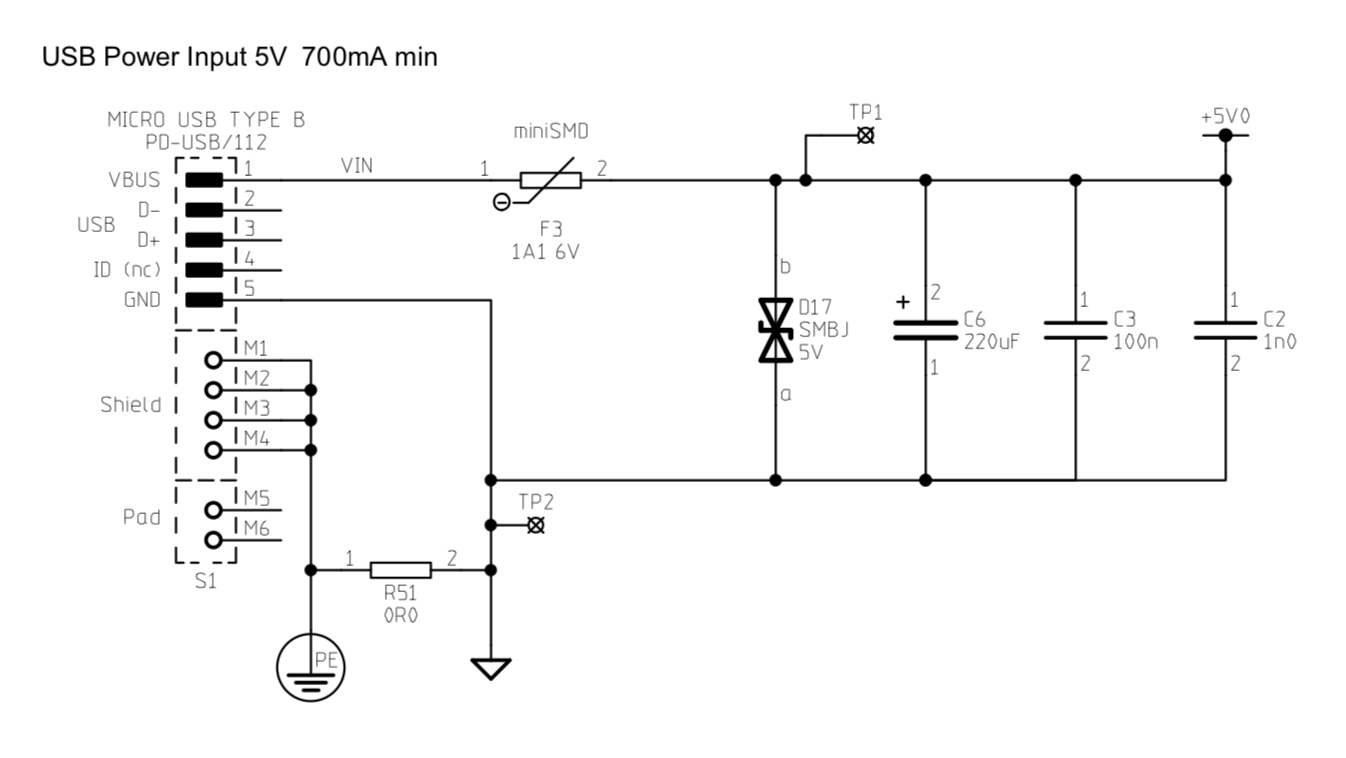
\includegraphics[scale=0.5]{obrazky/rpi_power.png}
  \end{center}
  \caption{Schéma napájení RPi přes USB, zdroj raspberrypi.org}
\end{figure}

\subsubsection{Napájení modulu SIM800}
Špičkový proudový odběr modulu SIM800 může dosahovat až 2 A při 5 V, zejména při registraci do sítě. Bude tedy nutné napájení dostatečně dimenzovat.

\begin{table}[h]
\centering
\caption{Proudový odběr komponent}
\label{my-label}
\begin{tabular}{|l|l|l|l|}
\hline
\textbf{Proudový odběr @5V {[}mA{]}} & \textit{min.} & \textit{typická} & \textit{max.} \\ \hline
RPi Zero W                       & 80               & 150              & 350          \\ \hline
RPi Camera v2.1                  & 100              & 100              & ?            \\ \hline
SIM800                           & 1,5              & -                & 2000         \\ \hline
PIR senzor                       & -                & -                & 65            \\ \hline
LED                              & -                & 400              & 420          \\ \hline
\end{tabular}
\end{table}

\subsubsection{Napájení výkonové LED}
Použitá výkonová LED dioda má proudový odběr 400 mA. Takový proud není možné poskytnout přes GPIO, bude nutné diodu spínat tranzistorovým spínačem. V úvahu ještě připadá spínat diodu pulzně přes PWM, ale bylo by nutné vyřešit problém s načasováním spouštění diody a pořizováním fotografií, aby nedocházelo ke stroboskopickému jevu.

\subsubsection{Návrh spínače výkonové LED}
Proudový odběr použité diody je 400 mA, úbytek napětí je 1,7 V. Diodu budeme spínat přes GPIO, které používá 3,3voltovou logiku. Prahové napětí pro sepnutí tranzistoru bude muset být minimálně 2,7 V, přičemž při napětím menším než 0,8 V musí být tranzistor zavřený. V úvahu připadá spínat LED diodu proudově řízeným bipolárním tranzistorem, nebo napěťově řízeným tranzistorem typu MOSFET. U tranzistoru typu MOSFET dochází k menším energetickým ztrátám než u bipolárního tranzistoru, ale vzhledem k vyšší ceně a malé dostupnosti výkonových logických tranzistorů pro 3,3voltovou logiku bude lepší použít Darlingtonovo zapojení bipolárních tranzistorů. Takový tranzistor má velké proudové zesílení a malý vstupní proud. 

V práci je použito tranzistorové pole ULN2003A sestávající ze sedmi Darlingtonových tranzistorů. K této součástce bylo přistoupeno z důvodu možného budoucího rozšíření o spínání více LED.  

\begin{figure}[h!]
  \begin{center}
    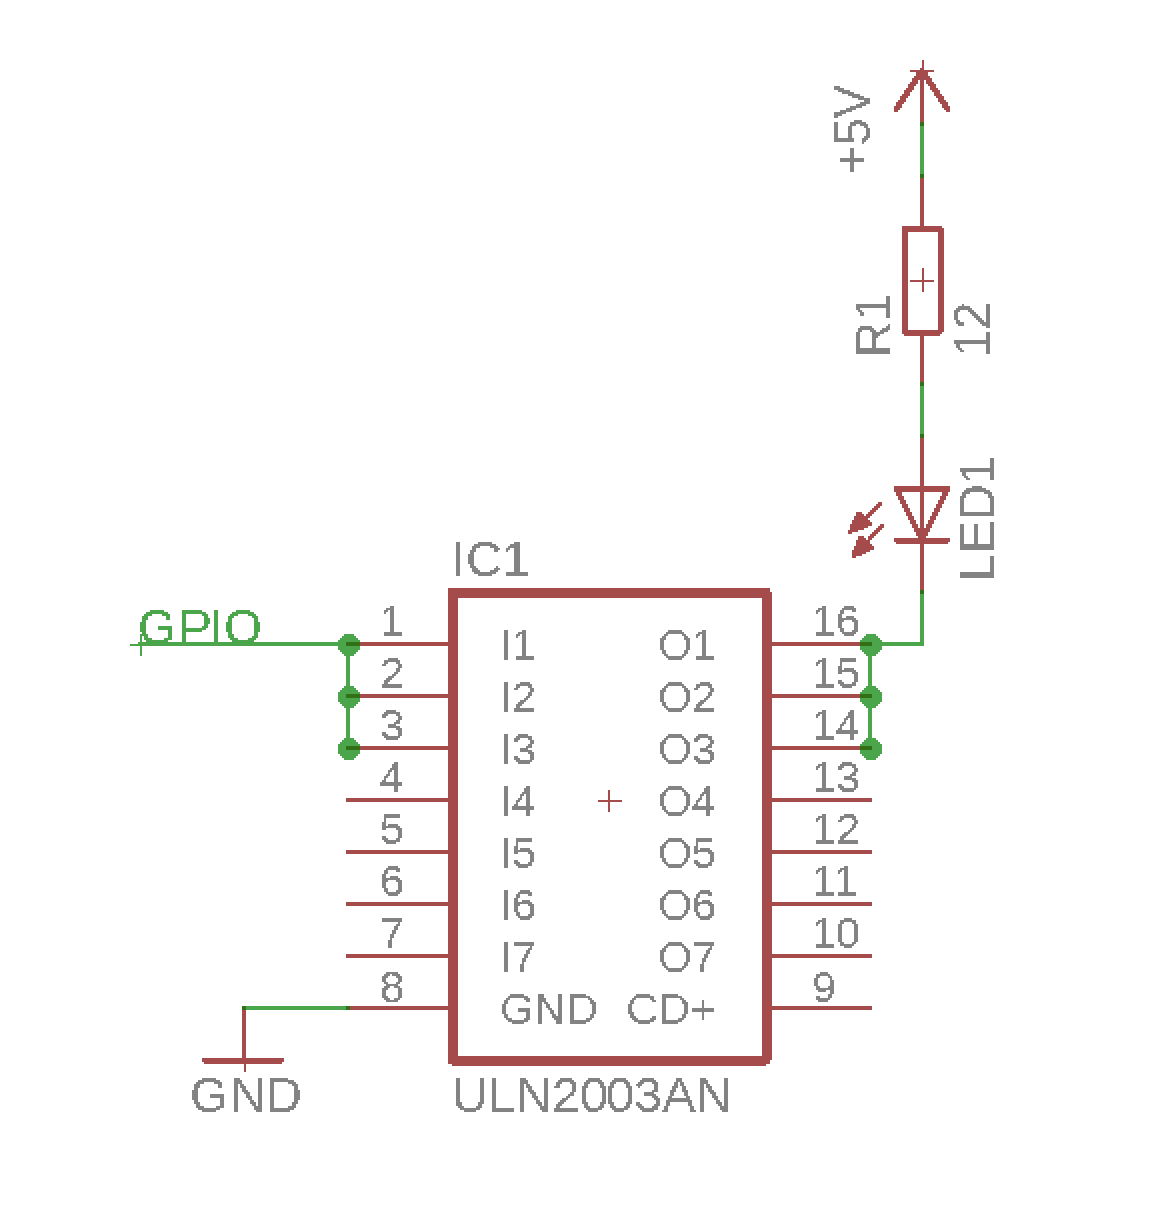
\includegraphics[scale=0.5]{obrazky/schema_switch2.png}
  \end{center}
  \caption{Schéma spínače výkonové LED}
\end{figure}


\subsection*{Solární panel a akumulátor}
Vzhledem k rozvaze o proudovém odběru jednotlivých komponent budeme vycházet z celkového průměrného proudového odběru 300 mA. Celkový příkon je tedy $0.3\times5 = 1.5 \ \jedn{W}$. Budeme uvažovat geografickou polohu Brna.

\subsubsection{Solární panel}
Dle Solargis.info dopadá v Brně 1150 $\jedn{kWh/m^2}$ solárního záření za rok.

$$1150000/8760 \approx 131 \ \jedn{W/m^2} $$

Průměrně tedy v Brně dopadá 131 $\jedn{W/m^2}$, avšak efektivita solárních panelů se pohybuje kolem 15\%, to je $20\ \jedn{W/m^2}$. Předpokládejme, že ztratíme dalších 33\% při přenosu energie. Celkově tedy máme využitelnou energie pouhých $14\ \jedn{W/m^2}$.

\subsubsection{Výpočet velikosti solárního panelu}
$$\frac{1.5\ \jedn{W}}{14\ \jedn{W/m^2}} \approx 1071 \ \jedn{cm^2}$$

Aby zařízení bylo možné provozovat celoročně, musíme provést výpočet velikosti solárního panelu pro měsíc s nejméně slunečnými dny, tedy pro prosinec. Využijeme kalkulátor Solar Electricity Handbook \cite{solar} pro zjištění úhrnu slunečního záření za měsíc prosinec.
Bude tedy nutné velikost panelu přepočítat s ohledem na měsíc prosinec. V prosinci v Brně dopadá průměrně 1,41 $\jedn{kWh/m^2}$ za den. Obecně platí, že panel by měl být natočen směrem na jih pod úhlem 41 stupňů pro celoroční optimum efektivity solárního panelu.


$$1410/24 \approx 59 \ \jedn{W/m^2} $$

Po přepočtu efektivity solárního panelu a ztráty při přenosu získáme $6 \ \jedn{W/m^2}$

\subsubsection{Přepočet výpočtu velikosti solárního panelu pro měsíc prosinec}
$$\frac{1.5W}{6\ \jedn{W/m^2}} \approx 2500 \ \jedn{cm^2}$$

Pro celoroční napájení bude nutné zajistit panel velikosti alespoň $2500 \ \jedn{cm^2}$

Tomuto požadavku odpovídá solární panel WS-30/12V.

\subsubsection{Akumulátor}

Použitý akumulátor musí zajistit nepřetržité napájení zařízení po dobu dlouhých zimních nocí, zejména v měsíci prosinci a také po dobu špatného počasí. Budeme tedy předpokládat, že zařízení musí vydržet týden bez dobíjení.

S ohledem na  nevýhody lithiových baterií uvedené v kapitol 1.5, bude zde vhodnější použít olověnou baterii.

Výpočítáme kapacitu akumulátoru pro noční provoz v prosinci, předpokládejme délku noci 16 h. Předpokládáme proudový odběr 300 mA při 5V.
$$16h\times0.3A=4.8 \ \jedn{Ah}$$

Výpočet kapacity akumulátoru pro týden bez slunce. Předpokládáme proudový odběr 300 mA při 5V.
$$7 dní \times 24 \ \jedn{h} \times 0.3 \ \jedn{A} \approx 50.4 \ \jedn{Ah}$$

Mezi odpovídající komerčně nabízené akumulátory patří Westinghouse WA12200 12V/20Ah.

\subsubsection{DC-DC Měnič 12/5V}
Pro změnu 12 V ze vstupu akumulátoru na 5 V, které je vyžadováno pro napájení všech komponent zařízení, je použit DC-DC měnič CPT 120503 12/5V od firmy Current Logic. Maximální udávaný proudový odběr je 3 A. Udávaná účinnost je v rozmezí 90 až 94 procent. Měnič také obsahuje ochranu proti zkratu a také ochranu proti přetížení.

\subsubsection{Solární regulátor Epsolar LS1024B}
Solární regulátor řídí nabíjení akumulátoru ze solárního panelu a také chrání baterii před jejím přebitím i hlubokým vybitím. Existují dva typy solárních regulátorů - MPPT a PWM. PWM solární regulátory vyhovují svými parametry pro naši aplikaci, používají pulzně šířkovou modulaci k dosažení optimálního nabití baterie. 

Požadavkem na solární regulátor je schopnost dodávat proud minimálně 3 A při 5 V, možnost připojení 12 V olověné baterie a 12 V solárního panelu. Dalším požadavkem je možnost vyčítání dat o stavu nabití baterie a nízká pořizovací cena. 

Tyto požadavky splňuje PWM solární regulátor LS1024B od firmy Epsolar, který umožňuje odebírat až 10A ze solárního panelu a dodávat 10A do zátěže. Je také umožněna datová komunikace přes protokol Modbus, realizovaná sériovou sběrnicí RS-485.

Komunikace mezi Raspberry Pi a solárním regulátorem je možné realizovat knihovnou epsolar-tracer pomocí převodníku RS-485 na USB.

\section{Komunikace s GSM modulem SIM800}
Komunikace s GSM modulem je realizována na rozhraní UART. Raspberry Pi disponuje jednou hardwarovou periferií UART, která je dostupná na pinech 14 (TX) a 15 (RX). Modul SIM800 podporuje maximální bitovou přenosovou rychlost 460800 bit/s, ale při použití multiplexovacího protokolu  GSM0710 je výrobcem doporučená maximální přenosová rychlost 115200 bit/s.

\subsubsection{Multiplexovací protkol GSM0710}
Modul SIM800 disponuje pouze jedním hardwarovým rozhraním UART, to znamená, že standardně můžeme otevřít pouze jedno spojení. V této aplikace, ale bude nutné navázat minimálně dvě spojení - pro PPP a druhé spojení pro posílání a přijímání SMS zpráv. 

3GPP definuje standard 27.010 (GSM0710), který umožňuje provádět multiplexování na přenosové vrstvě, které rozdělí datové toky do takzvaných DLC (Data Link Channel). Takový logický kanál je možné používat separátně, je tedy možné navázat PPP připojení na jednom kanálu a na druhém kanálu naslouchat zda-li nepřišla zpráva SMS.

Podpora pro multiplexovací protokol GSM0710 standardně v Linuxu není, ale je možné ji zkompilovat a přidat do kernelu v podobě LKM (Loadable Kernel Module). V repozitáři Linux kernelu ji najdeme v podobě zdrojového kódu jazyka C - n\_gsm.c. Po načtení modulu do kernelu je do adresáře proc přidán soubor zařízení gsmtty, který ale ještě není možný použít jako terminál.

Abychom mohli zařízení používat jako terminál je nutné připojit takzvanou "line discipline", toto je řešeno přes program cmux (autorem je Nicolas Le Munchet), který byl upraven dle specifikací modulu SIM800.

\begin{figure}[!h]
  \begin{center}
    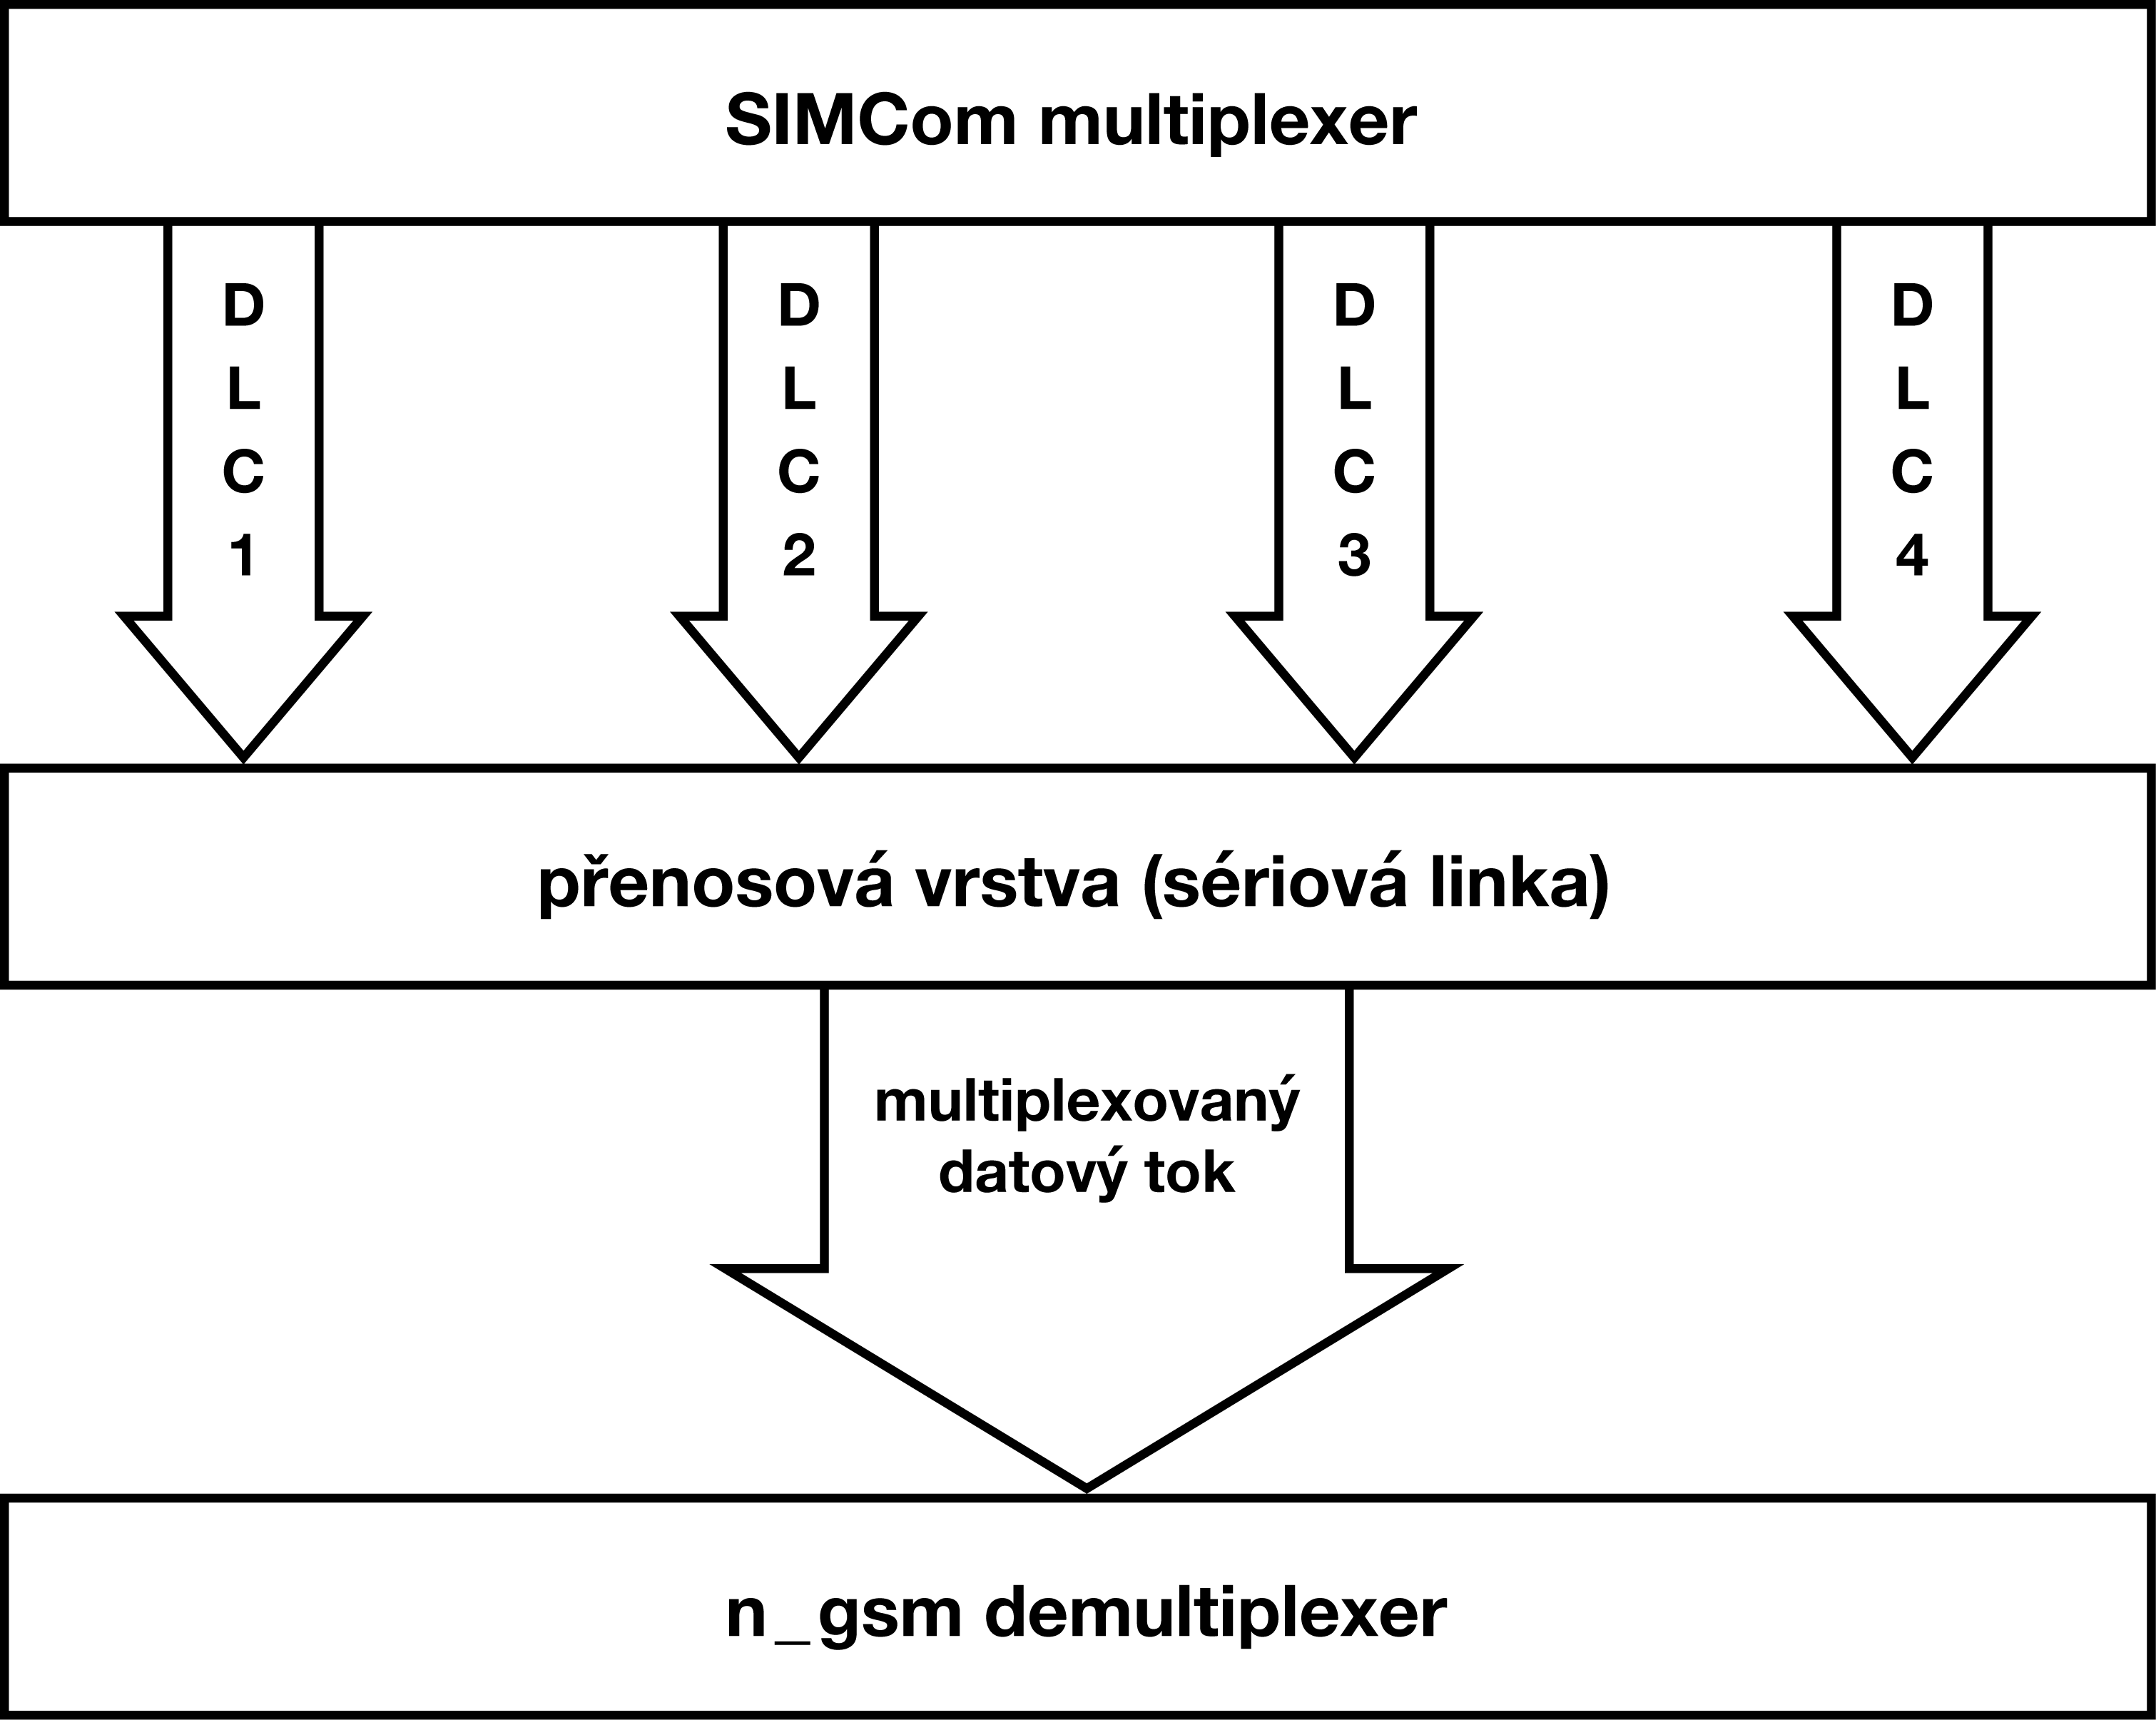
\includegraphics[scale=0.3]{obrazky/simcom.png}
  \end{center}
  \caption{Schéma multiplexovacího protokolu GSM0710}
\end{figure}

\clearpage

\section{Blokové schéma návrhu zařízení}
\begin{figure}[!h]
  \begin{center}
    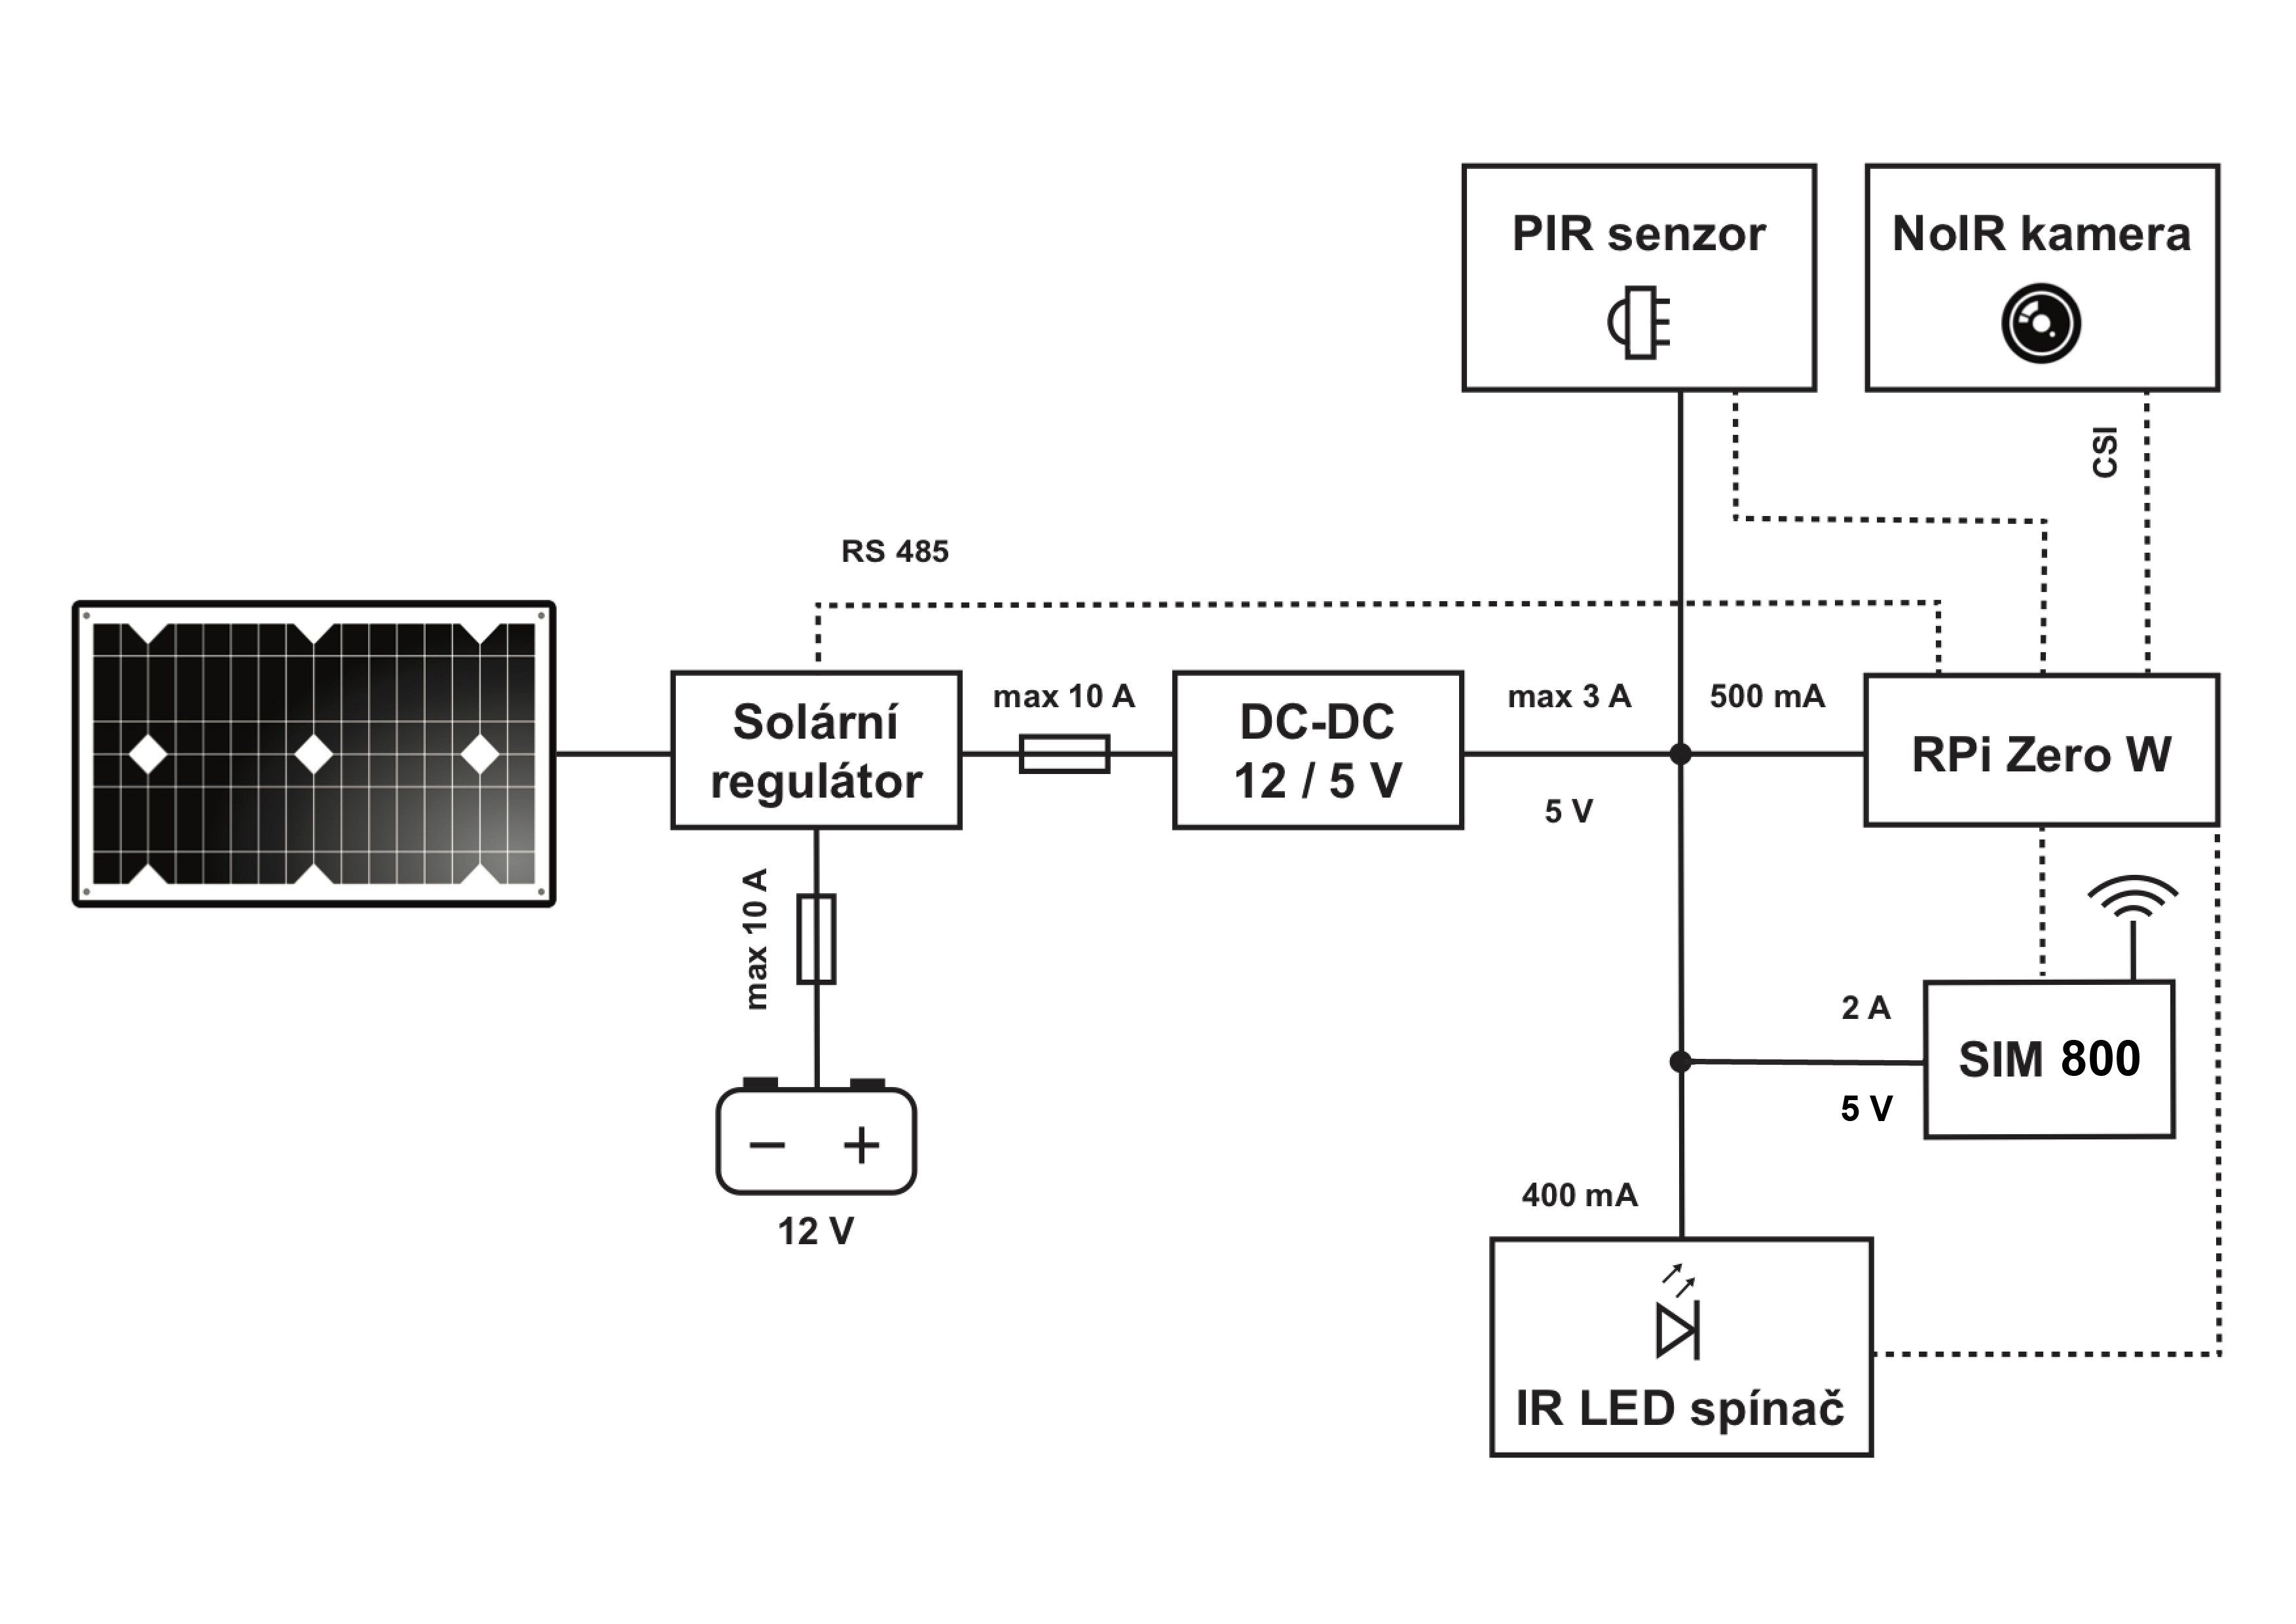
\includegraphics[scale=0.6, angle=90]{obrazky/blokove-schema-nove.png}
  \end{center}
  \caption{Blokové schéma návrhu zařízení}
\end{figure}

\clearpage

\section{Seznam a cena komponent}

\begin{table}[h]
\centering
\caption{Seznam komponent}
\label{komponenty}
\begin{tabular}{|l|l|l|}
\hline
\textbf{Jméno komponenty}                          & \textbf{Cena včetně DPH} \\ \hline
Raspberry Pi Zero W                                & 313 Kč (rpishop.cz)      \\ \hline
Raspberry Pi NoIR Camera Board V2                  & 858 Kč (rpishop.cz)      \\ \hline
SanDisk microSD karta 16 GB class 10                & 229 Kč (czc.cz)          \\ \hline
GSM/GPRS modul SIM800                              & 250 Kč                  \\ \hline
PIR modul HC-SR501                                 & 110 Kč (gme.cz)          \\ \hline
Výkonová IR LED dioda GT-P04IR4101                 & 45 Kč (gme.cz)           \\ \hline
Akumulátor Westinghouse WA12200                    & 1290 Kč (gme.cz)         \\ \hline
Solární panel WS-30/12V                            & 1990 Kč (gme.cz)         \\ \hline
Solární regulátor Epsolar LS1024B                  & 739 Kč (gme.cz)          \\ \hline
Převodník USB na RS-485                            & 240 Kč (rpishop.cz)        \\ \hline
DC/DC měnič 12V/5V CPT                             & 157 Kč                   \\ \hline
ULN20003A                                     & 10 Kč (gme.cz)           \\ \hline
Rezistor 22k                                       & 2,60 Kč (gme.cz)         \\ \hline
Drátový rezistor RD 12R 5W                         & 5,30 Kč (gme.cz)         \\ \hline
\end{tabular}
\end{table}

Cena komponent je platná k prosinci 2017.


%% Vložení souboru 'text/zaver' se závěrem
\chapter{Realizace a testování}

Praktickým výstupem práce je samotná realizace a otestování zařízení bez solárního napájení. Vybrané komponenty byly umístěny do plastové konstrukční krabičky, která byla upravena s ohledem na rozmístění jednotlivých komponent.

Na předním straně krabičky je čočka PIR senzoru, infračervená LED dioda a kamera. Na vrchní straně se nachází anténa pro GSM modul. 

Na pravém boku je 2.1 mm napájecí konektor. Je možné připojit akumulátor nebo stejnosměrný napájecí zdroj. Tolerované napájecí napětí je 8--20 V.

Dále se zde nachází tlačítko pro zapnutí čí vypnutí zařízení. Vypínání je řešeno softwarově, takže po stisku nedochází k úplnému vypnutí zařízení ale pouze k přepnutí do režimu halt. 


\begin{figure}[!h]
  \begin{center}
    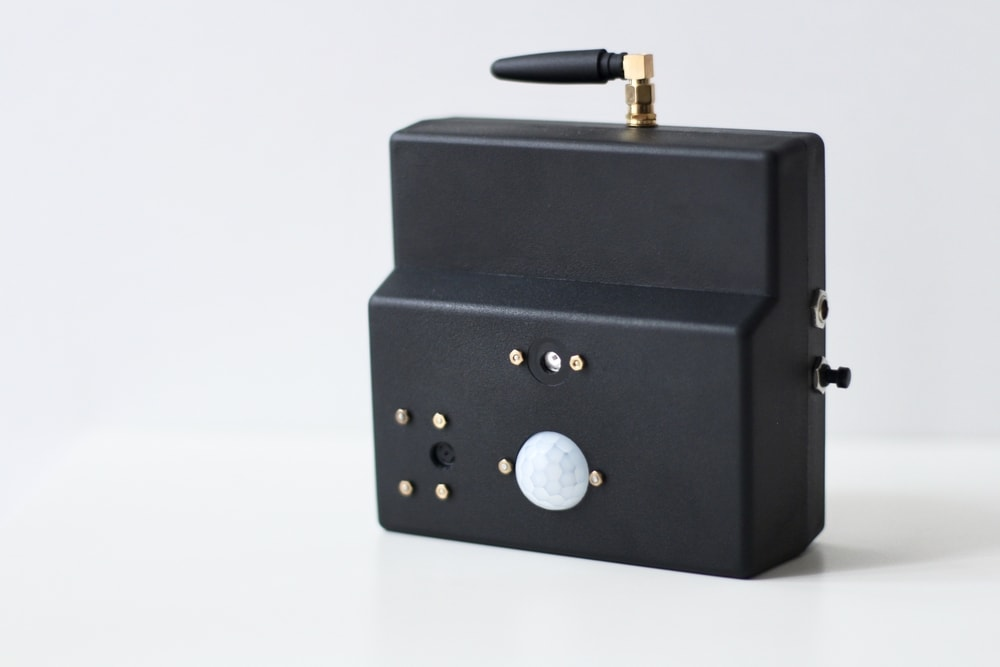
\includegraphics[scale=0.4]{obrazky/kamera.jpg}
  \end{center}
  \caption{Realizace kamerového zabezpečovacího systému}
\end{figure}


\begin{figure}[!h]
  \begin{center}
    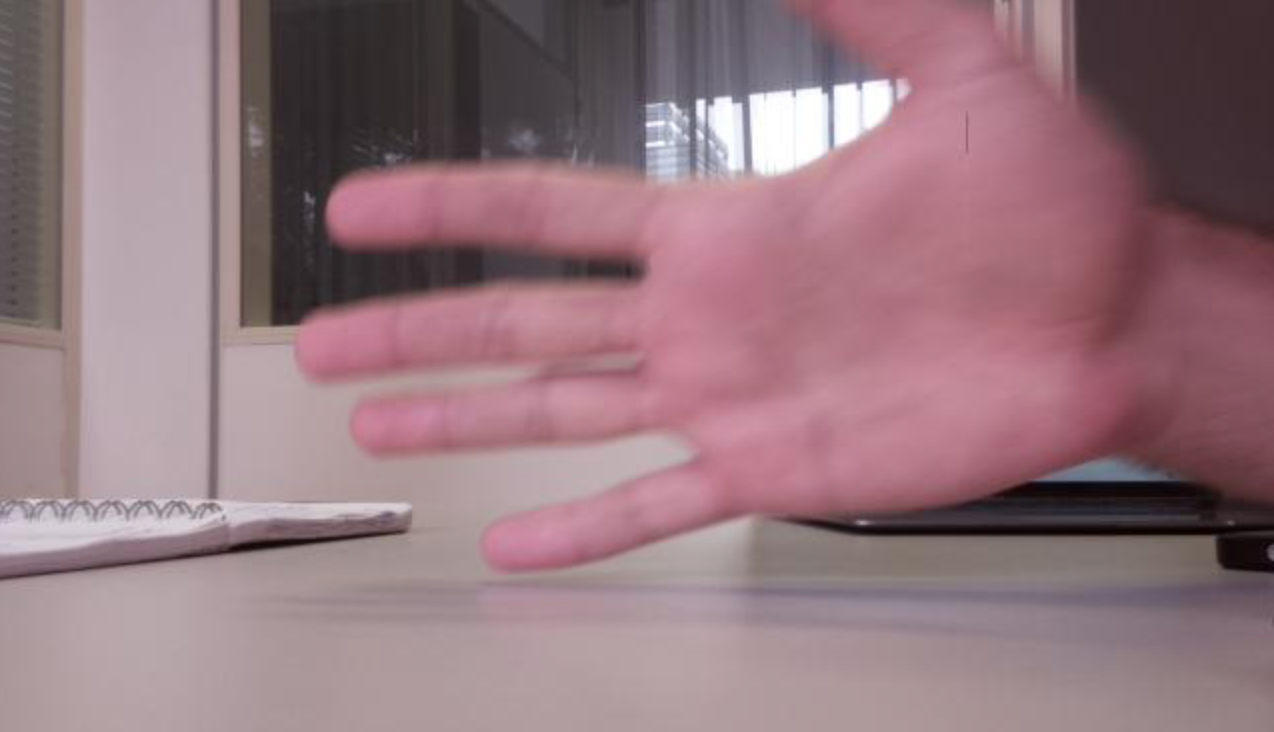
\includegraphics[scale=0.5]{obrazky/ukazka.png}
  \end{center}
  \caption{Ukázka denní fotografie pořízené kamerou}
\end{figure}

\begin{figure}[!h]
  \begin{center}
    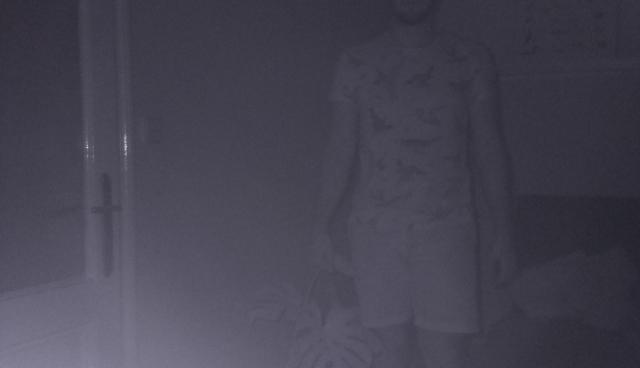
\includegraphics[scale=0.5]{obrazky/night_photo.jpg}
  \end{center}
  \caption{Ukázka noční fotografie pořízené kamerou s IR přísvitem}
\end{figure}

\clearpage

\section{Publikace aplikace}
Zdrojové kódy aplikace jsou spolu s dokumentací zveřejněny na serveru GitHub.

\href{www.github.com/marekvi95/bakalarka}{\textbf{www.github.com/marekvi95/bakalarka}}

\dirtree{%
 .1 /.
 .2 rpicameramon\DTcomment{hlavní modul}.
 .3 init.
 .3 motion.
 .3 config.
 .3 filemanipulation.
 .3 telemetry.
 .2 google\DTcomment{skripty na google API}.
 .3 scripts.
 .4 main.
 .4 index.
 .2 init\DTcomment{spouštění po startu}.
 .3 listen-shutdown.
 .2 docs\DTcomment{dokumentace aplikace}.
 .2 gsm\DTcomment{komunikace s gsm modulem}.
 }


\subsection*{Dokumentace}
K dokumentaci aplikace je použit generátor dokumentace Sphinx. Dokumentace ve zdrojovém kódu je realizována pomocí konvence Google docstring.

Dokumentace je napsaná v anglickém jazyce.


\chapter{Závěr}

V práci byla prozkoumána možná řešení a byl rámcově zpracován návrh kamerového zabezpečovacího systému založeného na minipočítači Raspberry Pi. 

V teoretické části práce byly vybrány hardwarové komponenty vhodné pro aplikaci na detekci pohybu s ohledem na co nejnižší spotřebu elektrické energie. Při výběru softwaru byl dáván důraz na jeho aktuálnost, otevřenost a rozšířitelnost. Z těchto důvodů byl pro práci vybrán jako hlavní programovací jazyk Python.  

V druhé kapitole je popsán návrh samotné aplikace pro detekci z obrazu a též za pomocí PIR senzoru. Důraz je kladen na konfigurovatelnost aplikace.

Třetí kapitola se věnuje návrhu napájení jednotlivých komponent pomocí solárního panelu a akumulátoru.

Poslední kapitola se věnuje realizaci zařízení a testování funkčnosti.

\section{Možná vylepšení}
Praktická realizace zařízení ukázala nedostatky při použití minipočítače Raspberry Pi. Vzhledem k požadavku na bateriové napájení se jako vhodnější jeví použití mikrokontroléru s podporou uspávání, které by pomohlo ušetřit energii v době neaktivity zařízení. Další možností je například implementace detektoru pohybu na FPGA. Tato možnost by mohla přinést nižší nároky na napájení a také rychlejší a spolehlivější zpracování obrazu.

Za zvážení by také stálo použití kamery s lepším objektivem, který by umožnil pořizovat kvalitnější fotografie.

Pro připojení k sítí Internet by bylo vhodnější použít modul podporující sítě čtvrté generace. Nástupce modelu SIM800 je SIM7100 od firmy Simcomm, který podporuje i nový standard úzkopásmového LTE NB IoT. V takovém případě by nebylo nutné provádět úpravy ve stávajícím softwaru.

Co se týká aplikace pro detekci, tak jako možné vylepšení se nabízí lokalizace a klasifikace objektu, tak aby bylo možné rozeznávat, zda se jedná o člověka nebo o zvíře. Případná další vylepšení by mohla přinést aplikace neuronových sítí.







%% Vložení souboru 'text/literatura' se seznamem literatury
% Pro sazbu seznamu literatury použijte jednu z následujících možností

%%%%%%%%%%%%%%%%%%%%%%%%%%%%%%%%%%%%%%%%%%%%%%%%%%%%%%%%%%%%%%%%%%%%%%%%%
%1) Seznam citací definovaný přímo pomocí prostředí literatura / thebibliography

\begin{literatura}{99}
	
\bibitem{rpidoc}
		Raspberry Pi Foundation:
    \emph{Oficiální dokumentace k Raspberry Pi}\/ [online].
    Dostupné z~URL:\\
    <\url{https://www.raspberrypi.org/documentation/}>.
    
\bibitem{cameradoc}
		Camera Python interface documentation:
    \emph{Oficiální dokumentace k Picamera}\/ [online].
    Dostupné z~URL:\\
    <\url{http://picamera.readthedocs.io}>.

\bibitem{bechnik_2014}
    BECHNÍK B.
    \emph{Stručná historie fotovoltaiky}\/ [online].
    2014, poslední aktualizace 1.\,9.\,2014 [cit. 18.\,11.\,2017].
    Dostupné z~URL:
    \(<\)\url{http://oze.tzb-info.cz/fotovoltaika/11652-strucna-historie-fotovoltaiky}\(>\)

\bibitem{fbmi_video}
    ČVUT Praha - Fakulta biomedicínského inženýrství
    \emph{Detekce pohybu ve videu}\/ [online].
    [cit. 1.\,10.\,2017].
    Dostupné z~URL:
    \(<\)\url{http://fbmi.cvut.cz/files/predmety/3528/public/Detekce\%20pohybu\%20ve\%20videu.pdf}\(>\)

\bibitem{pir_senzor}
    MICHALEC L.
    \emph{PIR detektor: skvělý sluha, ale zlý pán}\/ [online].
    2013, poslední aktualizace 18.\,3.\,2013 [cit. 1.\,10.\,2017].
    Dostupné z~URL:
    \(<\)\url{https://vyvoj.hw.cz/automatizace/pir-cidlo-skvely-sluha-ale-zly-pan.html}\(>\)

\bibitem{solargis}
		Solargis
    \emph{Mapy globálního horizontálního solárního záření pro Českou republiku}\/ [online].
    Dostupné z~URL:\\
    <\url{https://solargis.com/products/maps-and-gis-data/free/download/czech-republic}>.

\bibitem{sony}
    HUFKENS K.
    \emph{Spektrální citlivost Raspberry Pi kamery}\/ [online].
    2016, poslední aktualizace 5.\,6.\,2016 [cit. 1.\,10.\,2017].
    Dostupné z~URL:
    \(<\)\url{http://www.khufkens.com/2016/06/05/raspberry-pi-camera-v2-spectral-response-curve/}\(>\)
    
\bibitem{solar}
    BOXWELL M.
    \emph{Tabulky solárního záření pro danou lokaci}\/ [online].
    2017, [cit. 18.\,11.\,2017].
    Dostupné z~URL:
    \(<\)\url{http://www.solarelectricityhandbook.com/solar-irradiance.html}\(>\)
    
    

\end{literatura}


%%%%%%%%%%%%%%%%%%%%%%%%%%%%%%%%%%%%%%%%%%%%%%%%%%%%%%%%%%%%%%%%%%%%%%%%%
%%2) Seznam citací pomocí BibTeXu
%% Při použití je nutné v TeXnicCenter ve výstupním profilu aktivovat spouštění BibTeXu po překladu.
%% Definice stylu seznamu
%\bibliographystyle{unsrturl}
%% Pro českou sazbu lze použít styl czechiso.bst ze stránek
%% http://www.fit.vutbr.cz/~martinek/latex/czechiso.tar.gz
%%\bibliographystyle{czechiso}
%% Vložení souboru se seznamem citací
%\bibliography{text/literatura}
%
%% Následující příkaz je pouze pro ukázku sazby literatury při použití BibTeXu.
%% Způsobí citaci všech zdrojů v souboru odkazy.bib, i když nejsou citovány v textu.
%\nocite{*}

%% Vložení souboru 'text/zkratky' se seznam použitých symbolů, veličin a zkratek
\begin{seznamzkratek}{KolikMista}
\novazkratka{IoT}%
{IoT}%
{Internet of Things, Internet věcí}

\novazkratka{SoC}%
{SoC}%
{System on a chip}

\novazkratka{HDMI}%
{HDMI}%
{Rozhraní pro přenos videa a zvuku}

\novazkratka{FPS}%
{FPS}%
{Počet snímků za sekundu}

\novazkratka{GPIO}%
{GPIO}%
{General Purpose Input Output}

\novazkratka{UART}%
{UART}%
{Universal asynchronous receiver-transmitter}

\novazkratka{SPI}%
{SPI}%
{Serial Peripheral Interface Bus}

\novazkratka{I2C}%
{I2C}%
{Inter-Integrated Circuit}

\novazkratka{PCM}%
{PCM}%
{Pulzně kódová modulace}

\novazkratka{PWM}%
{PWM}%
{Pulzně šířková modulace}

\novazkratka{DMA}%
{DMA}%
{Direct Memory Access, tj. přímý přístup do paměti}

\novazkratka{NoIR}%
{NoIR}%
{No Infrared, označení pro kameru bez IR filtru}

\novazkratka{CMOS}%
{CMOS}%
{technologie výroby integrovaných obvodů}

\novazkratka{GSM}%
{GSM}
{standard pro mobilní hlasovou komunikaci}%

\novazkratka{GPRS}%
{GPRS}%
{rozšíření GSM o paketová data}

\novazkratka{PPP}%
{PPP}%
{Point-to-Point Protocol}

\novazkratka{APN}%
{APN}
{Access Point Name}%



\novazkratka{PIR}%
{PIR}%
{Passive Infrared Sensor}


\novazkratka{PIL}%
{PIL}%
{Python Imaging Library}


\novazkratka{API}%
{API}%
{Application Programmable Interface}


\novazkratka{BSD}%
{BSD}%
{Berkeley Software Distribution}


\novazkratka{JSON}%
{JSON}%
{JavaScript Object Notation}


\novazkratka{FET}%
{FET}%
{Field-effect transistor}


\novazkratka{}%
{}%
{}



\end{seznamzkratek}


%% Začátek příloh
\prilohy

%% Vysázení seznamu příloh
\seznampriloh

%% Vložení souboru 'text/prilohy' s přílohami
\chapter{Zapojení GPIO pinů na Raspberry Pi}
\begin{table}[h]
\centering
\caption{Zapojení GPIO pinů na Raspberry Pi}
\label{gpio}
\begin{tabular}{|l|l|l|l|l|l|l|l|}
\hline
\textbf{zapojení} & \textbf{název} & \textbf{BCM} & \textbf{pin} & \textbf{pin} & \textbf{BCM} & \textbf{název} & \textbf{zapojení} \\ \hline
-                 & 3v3            & -            & 1            & 2            & -            & 5V             & Napájení                \\ \hline
-                 & SDA            & 2            & 3            & 4            & -            & 5V             & -                 \\ \hline
 Tlačítko ON/OFF  & SCL            & 3            & 5            & 6            & -            & GND            & GND                 \\ \hline
 SIM800 RST       & GPCLK0         & 4            & 7            & 8            & 14           & TXD            & SIM800 Rx         \\ \hline
-                 & GND            & -            & 9            & 10           & 15           & RXD            & SIM800 Tx         \\ \hline
-                 &                & 17           & 11           & 12           & 18           & PWM0           & PIR signál        \\ \hline
-                 &                & 27           & 13           & 14           & -            & GND            & -                 \\ \hline
-                 &                & 22           & 15           & 16           & 23           &                & LED signál        \\ \hline
-                 & 3v3            & -            & 17           & 18           & 24           &                & -                 \\ \hline
-                 & MOSI           & 10           & 19           & 20           & -            & GND            & -                 \\ \hline
-                 & MISO           & 9            & 21           & 22           & 25           &                & -                 \\ \hline
-                 & SCLK           & 11           & 23           & 24           & 8            & CE0            & -                  \\ \hline
-                 & GND            & -            & 25           & 26           & 7            & CE1            & -                  \\ \hline
-                 & ID\_SD         & 0            & 27           & 28           & 1            & ID\_SC         & -                 \\ \hline
-                 &                & 5            & 29           & 30           & -            & GND            & -                 \\ \hline
-                 &                & 6            & 31           & 32           & 12           & PWM0           & -                 \\ \hline
-                 & PWM1           & 13           & 33           & 34           & -            & GND            & -                 \\ \hline
-                 & MISO           & 19           & 35           & 36           & 16           &                & -                  \\ \hline
-                 &                & 26           & 37           & 38           & 20           & MOSI           & -                  \\ \hline
-                 & GND            & -            & 39           & 40           & 21           & SCLK           & -                 \\ \hline
\end{tabular}
\end{table}

\chapter{Denní úhrn solárního záření v Brně}
\begin{figure}[!h]
  \begin{center}
    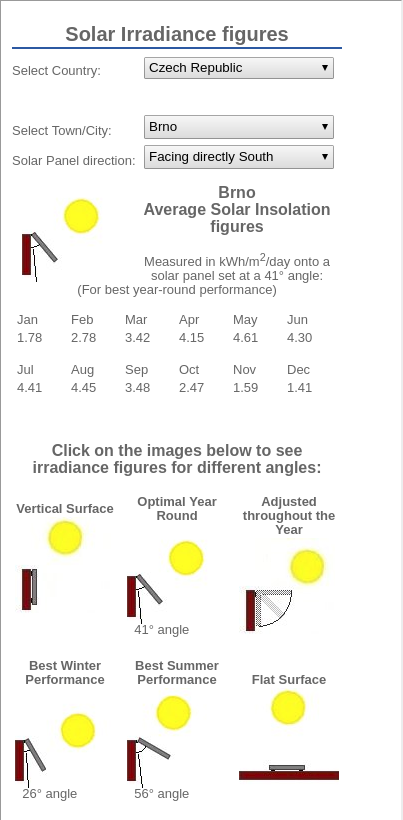
\includegraphics[scale=0.61]{obrazky/solar-irradiance-Brno.png}
  \end{center}
  \caption{Solar Irradiance Brno \cite{solar}}
\end{figure}


\chapter{Dokumentace aplikace}


\setboolean{@twoside}{false}
\shorthandoff{-}
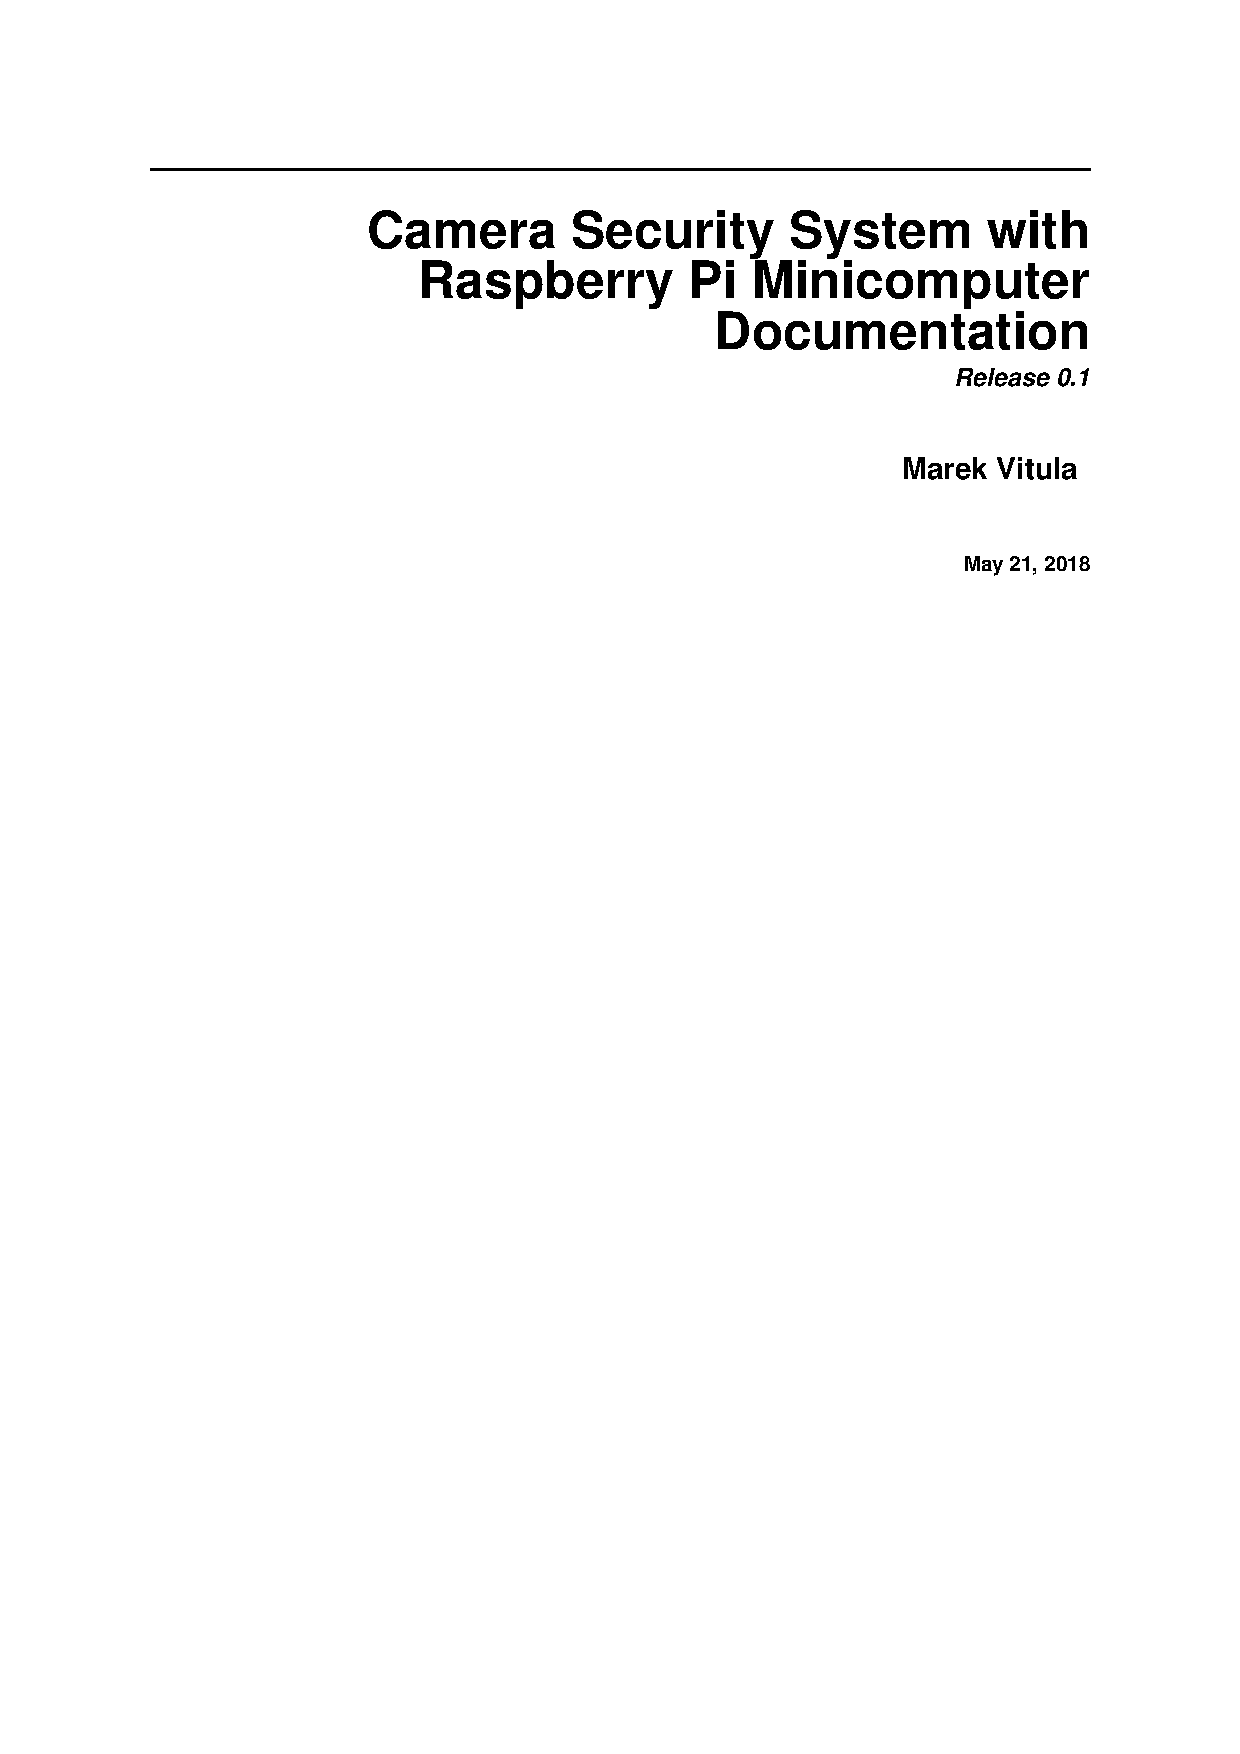
\includepdf[pages=-]{pdf/dokumentace}
\shorthandon{-}

%% Konec dokumentu
\end{document}

